\chapter{LHC-ATLAS実験}\label{chapter2}

LHC-ATLAS実験とは、Large Hadron Collider~(LHC)~\cite{article:LHC}を用いた高エネルギーの陽子–陽子衝突によって生成された粒子をATLAS~(A Troidal LHC ApparatuS)検出器によって検出し、標準模型の精密測定や新粒子探索などを行う実験である~\cite{Aad:1129811}。
LHCは2018年に第2期運転~(Run-2)を終了し、2019年から2021年にかけてLHC及びATLAS検出器のアップグレードが行われ、2022年7月からはRun-3として運転を再開している。

本章では、Run-3におけるLHC及びATLAS検出器の概要とATLAS実験で採用されているトリガーシステムについて述べる。

\section{LHC加速器}
\label{section2-1}
Large Hadron Collider~(LHC)は、スイスのジュネーブ郊外にある欧州素粒子原子核研究機構~(CERN)~\cite{article:CERN}の地下に建設された周長約27~km の世界最大の大型ハドロン衝突型加速器である。LHCの全体像を図~\ref{fig:LHC_overview}に示す。
%\cite{article:Overall_view_LHC}。
LHCは重心系エネルギー14~TeV、瞬間ルミノシティ$1.0\times10^{34}$~cm$^{-2}$s$^{-1}$で陽子陽子衝突が可能なように設計されている。
ここで、ルミノシティとは衝突型加速器における粒子同士の衝突頻度を表している。瞬間ルミノシティが毎秒あたりの衝突頻度、時間で積分したものが積分ルミノシティと定義され、観測されるデータ量はこの積分ルミノシティに比例する。

LHCは陽子ビームが反対方向に周回するための2つのリングから構成されており、4か所ある衝突点にそれぞれ検出器が設置されている。
その衝突点の一つにATLAS検出器が設置され、陽子陽子衝突から生成される粒子を検出する。
他3か所にも検出器が設置されており、それぞれCMS~(Compact Muon Solenoid)~\cite{article:CMSExperiment}、LHCb~(Large Hadron Collider b)~\cite{article:LHCbExperiment}、ALICE~(A Large Ion Collider Experiment)~\cite{article:ALICEExperiment}である。
ATLASとCMSの2つの検出器は、標準模型の検証から標準模型を超える現象の探索まで可能な汎用検出器である。
LHCb~と呼ばれる検出器は、$B$--ハドロン系の物理を研究するために設計されたものである。
最後のALICEは、QCD現象を探るために重イオン衝突の研究に最適化された検出器である。


\begin{figure}[tb]
  \centering
  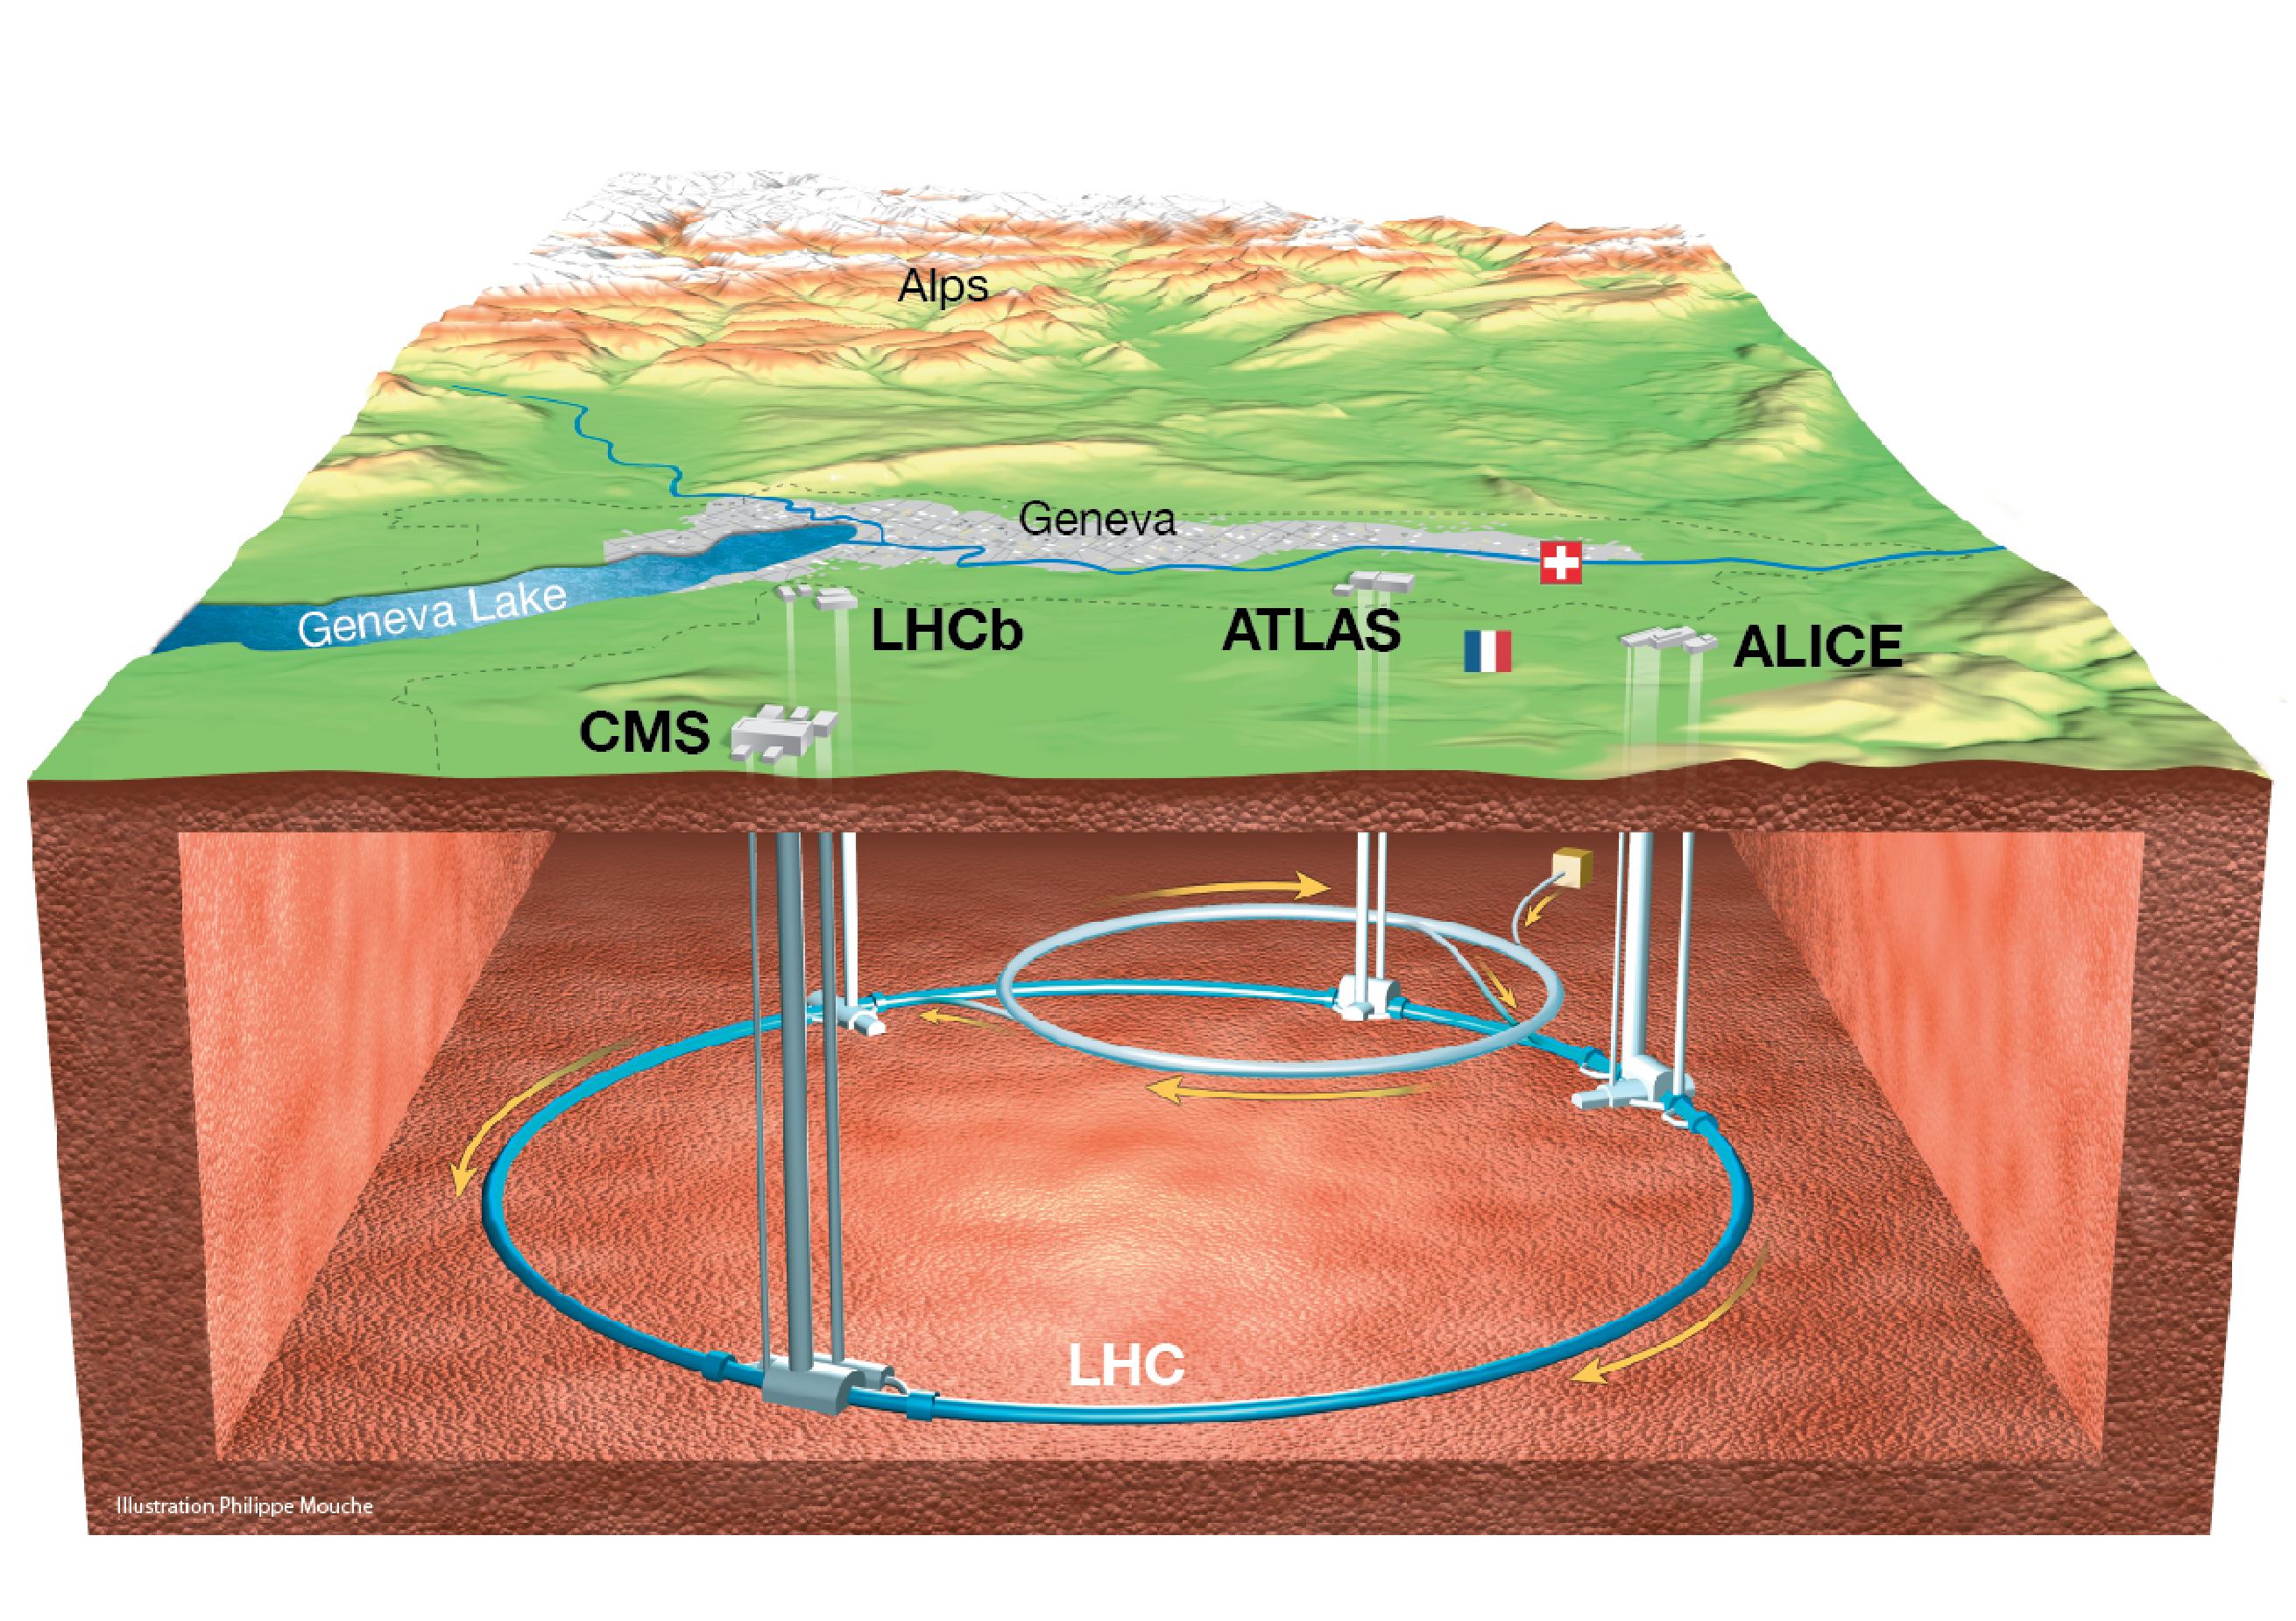
\includegraphics[clip, width=14cm]{fig/2/LHC_overview.pdf}
  \caption{LHC加速器の全体図\cite{article:Overall_view_LHC}。地下100mに設置されたLHCの4つの衝突点に ATLAS、CMS、ALICE、LHCb などの検出器が配置されている。}
  \label{fig:LHC_overview}
\end{figure}

\begin{figure}[tb]
  \centering
  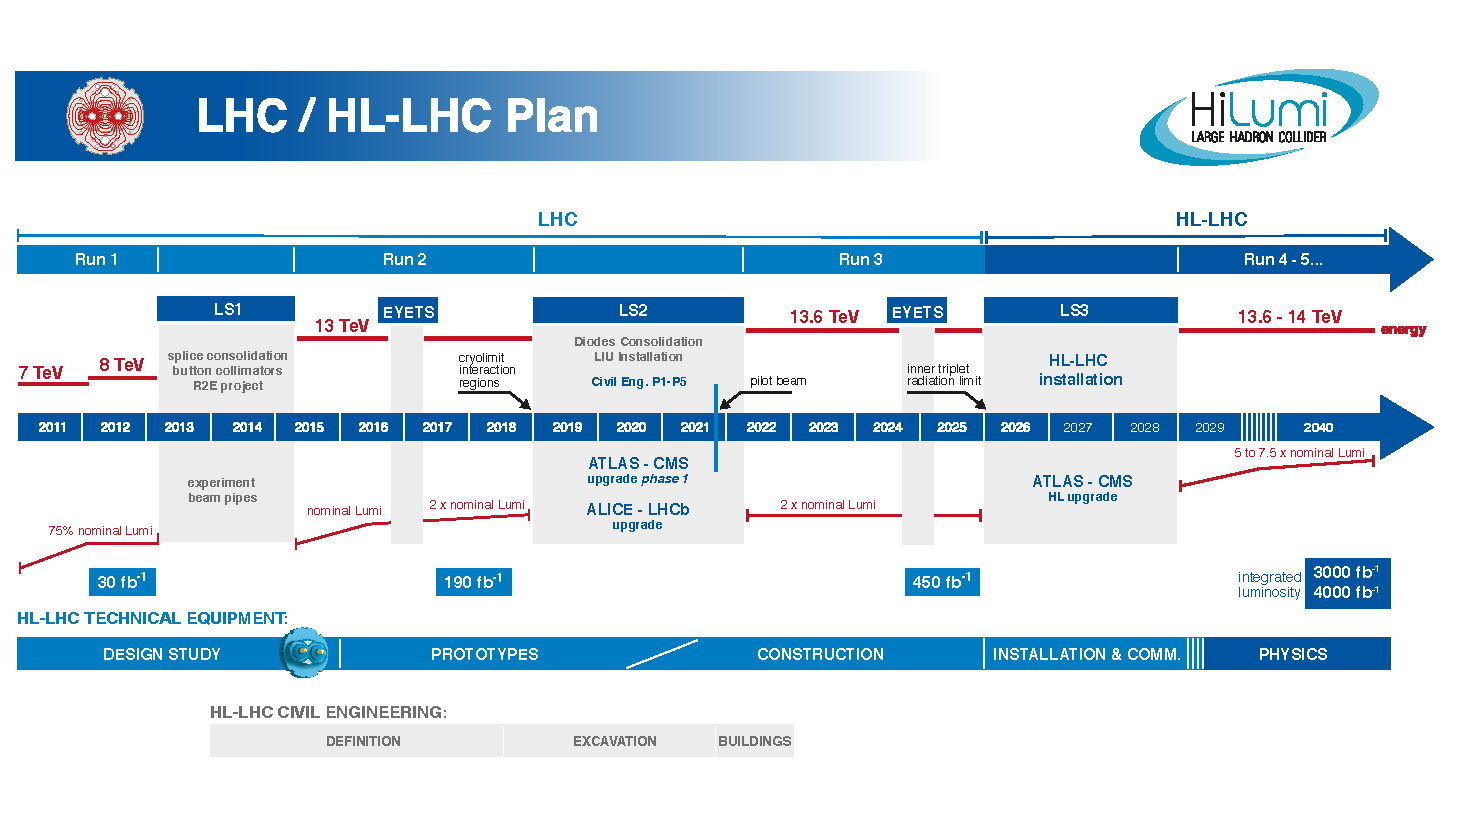
\includegraphics[clip, width=15cm]{fig/1/HL-LHC_Janvier2022.pdf}
  \caption{LHC 加速器の運転とアップグレード計画\cite{article:LHCDesignReport}。LHCでは2019年から2022年初旬までの間にPhase-1 Upgradeが行われ、現在はRun-3として運転を再開している。}
  \label{fig:LHC_Plan}
\end{figure}

図~\ref{fig:LHC_Plan}にLHC加速器の運転計画を示す。LHCは2010年から本格的に実験を開始し、2010年から2012年にかけて行われた運転を\mbox{Run-1}、2015年から2018年にかけて行われた運転をRun-2と呼ぶ。
 \mbox{Run-1}では重心系エネルギー7-8~TeV、瞬間最高ルミノシティ$0.77\times10^{34}$~cm$^{-2}$s$^{-1}$での運転を行い、Run-2では重心系エネルギー13~TeV、瞬間最高ルミノシティ$2.0\times10^{34}$~cm$^{-2}$s$^{-1}$での運転を行った。
2019年から2022年初旬までのLong Shutdown 2~(LS2)の期間に加速器のアップグレードが行われ、2022年7月から2025年にかけて行われるRun-3では陽子陽子衝突の重心系エネルギーを 13.6~TeV、瞬間ルミノシティ2.0$\times$10$^{34}$~cm$^{-2}$s$^{-1}$での運転を行い、Run-2で取得したデータと合わせて積分ルミノシティ350~fb$^{-1}$のデータを取得する予定である。さらにその後、アップグレードを経て2029年からはより高いルミノシティでの高輝度LHC-ATLAS実験(HL-LHC)の運転が予定されている。


\begin{figure}[tb]
  \centering
  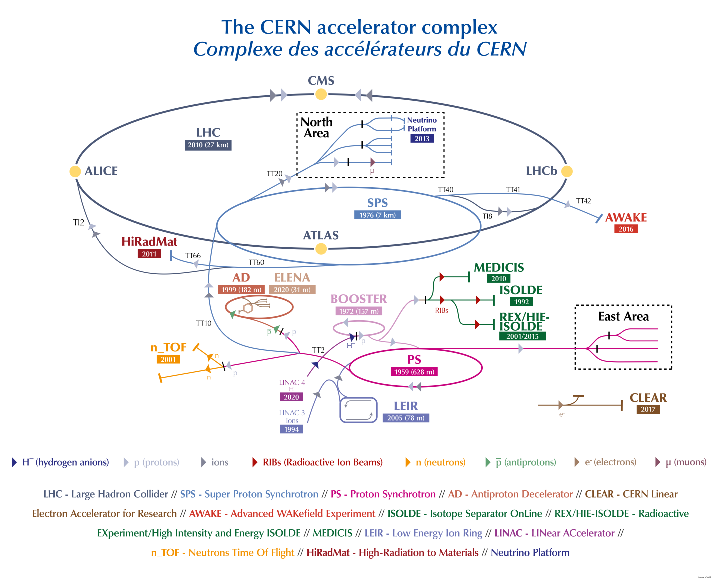
\includegraphics[clip, width=14cm]{fig/2/CCC-v2022.pdf}
  \caption{CERN に設置されている加速器群\cite{article:accelerator-complex}。}
  \label{fig:LHC加速器}
\end{figure}


LHCでは陽子を衝突させるまでに、いくつかの前段加速器を使用しTeVスケールのエネルギーまで陽子を加速している。図~\ref{fig:LHC加速器}に概略図を示す。
初めに負水素イオン(H$^-$、水素原子に電子を加えたもの)を線形加速器であるLINAC4~\cite{article:Linearaccelerator4}で160~MeVまで加速する。次に、強い電場をかけることで負水素イオンから2個の電子を剥ぎ取り、陽子だけの状態にする。そして、Proton Synchrotron~Booster~(PSB)~\cite{article:TheProtonSynchrotronBooster}に入射し 1.4~GeVまで加速された後、Proton~Synchrotron~(PS)~\cite{article:TheProtonSynchrotron}で陽子を26~GeVまで加速し、40~MHzのバンチ構造を持った陽子ビームを形成する。
その後、Super Proton Synchrotron~(SPS)~\cite{article:TheSuperProtonSynchrotron}で450~GeVまで加速された後、陽子ビームはLHCに入射され最大で7~TeVまで加速される。
陽子ビームは25~nsのバンチ間隔で入射されているため、陽子陽子衝突を起こす際の各バンチの衝突頻度は40~MHzとなっている。



\section{LHC-ATLAS 実験}\label{section2-2}
%本節では、LHC-ATLAS 実験で使用されるATLAS 検出器とATLAS 実験で使用されているトリガーシステムについて説明する。

%\subsection{ATLAS検出器}
ATLAS検出器は、LHCの衝突点の1つに設置された、直径25m、長さ44mの円筒形の大型汎用検出器である\cite{Aad:1129811}。ATLAS 検出器の全体像を図~\ref{fig:ATLAS検出器}に示す。
ATLAS検出器は複数の検出器を組み合わせて構成されており、内側から内部飛跡検出器、カロリメータ、ミューオン検出器といった検出器が設置されている。また、内部飛跡検出器とカロリメータの間には超伝導ソレノイド磁石、カロリメータの外側にはトロイド磁石がそれぞれ設置されている。
これらの検出器から得られる情報を組み合わせることで、粒子識別や粒子のエネルギーなどの測定を行っている。

\begin{figure}[tb]
  \centering
  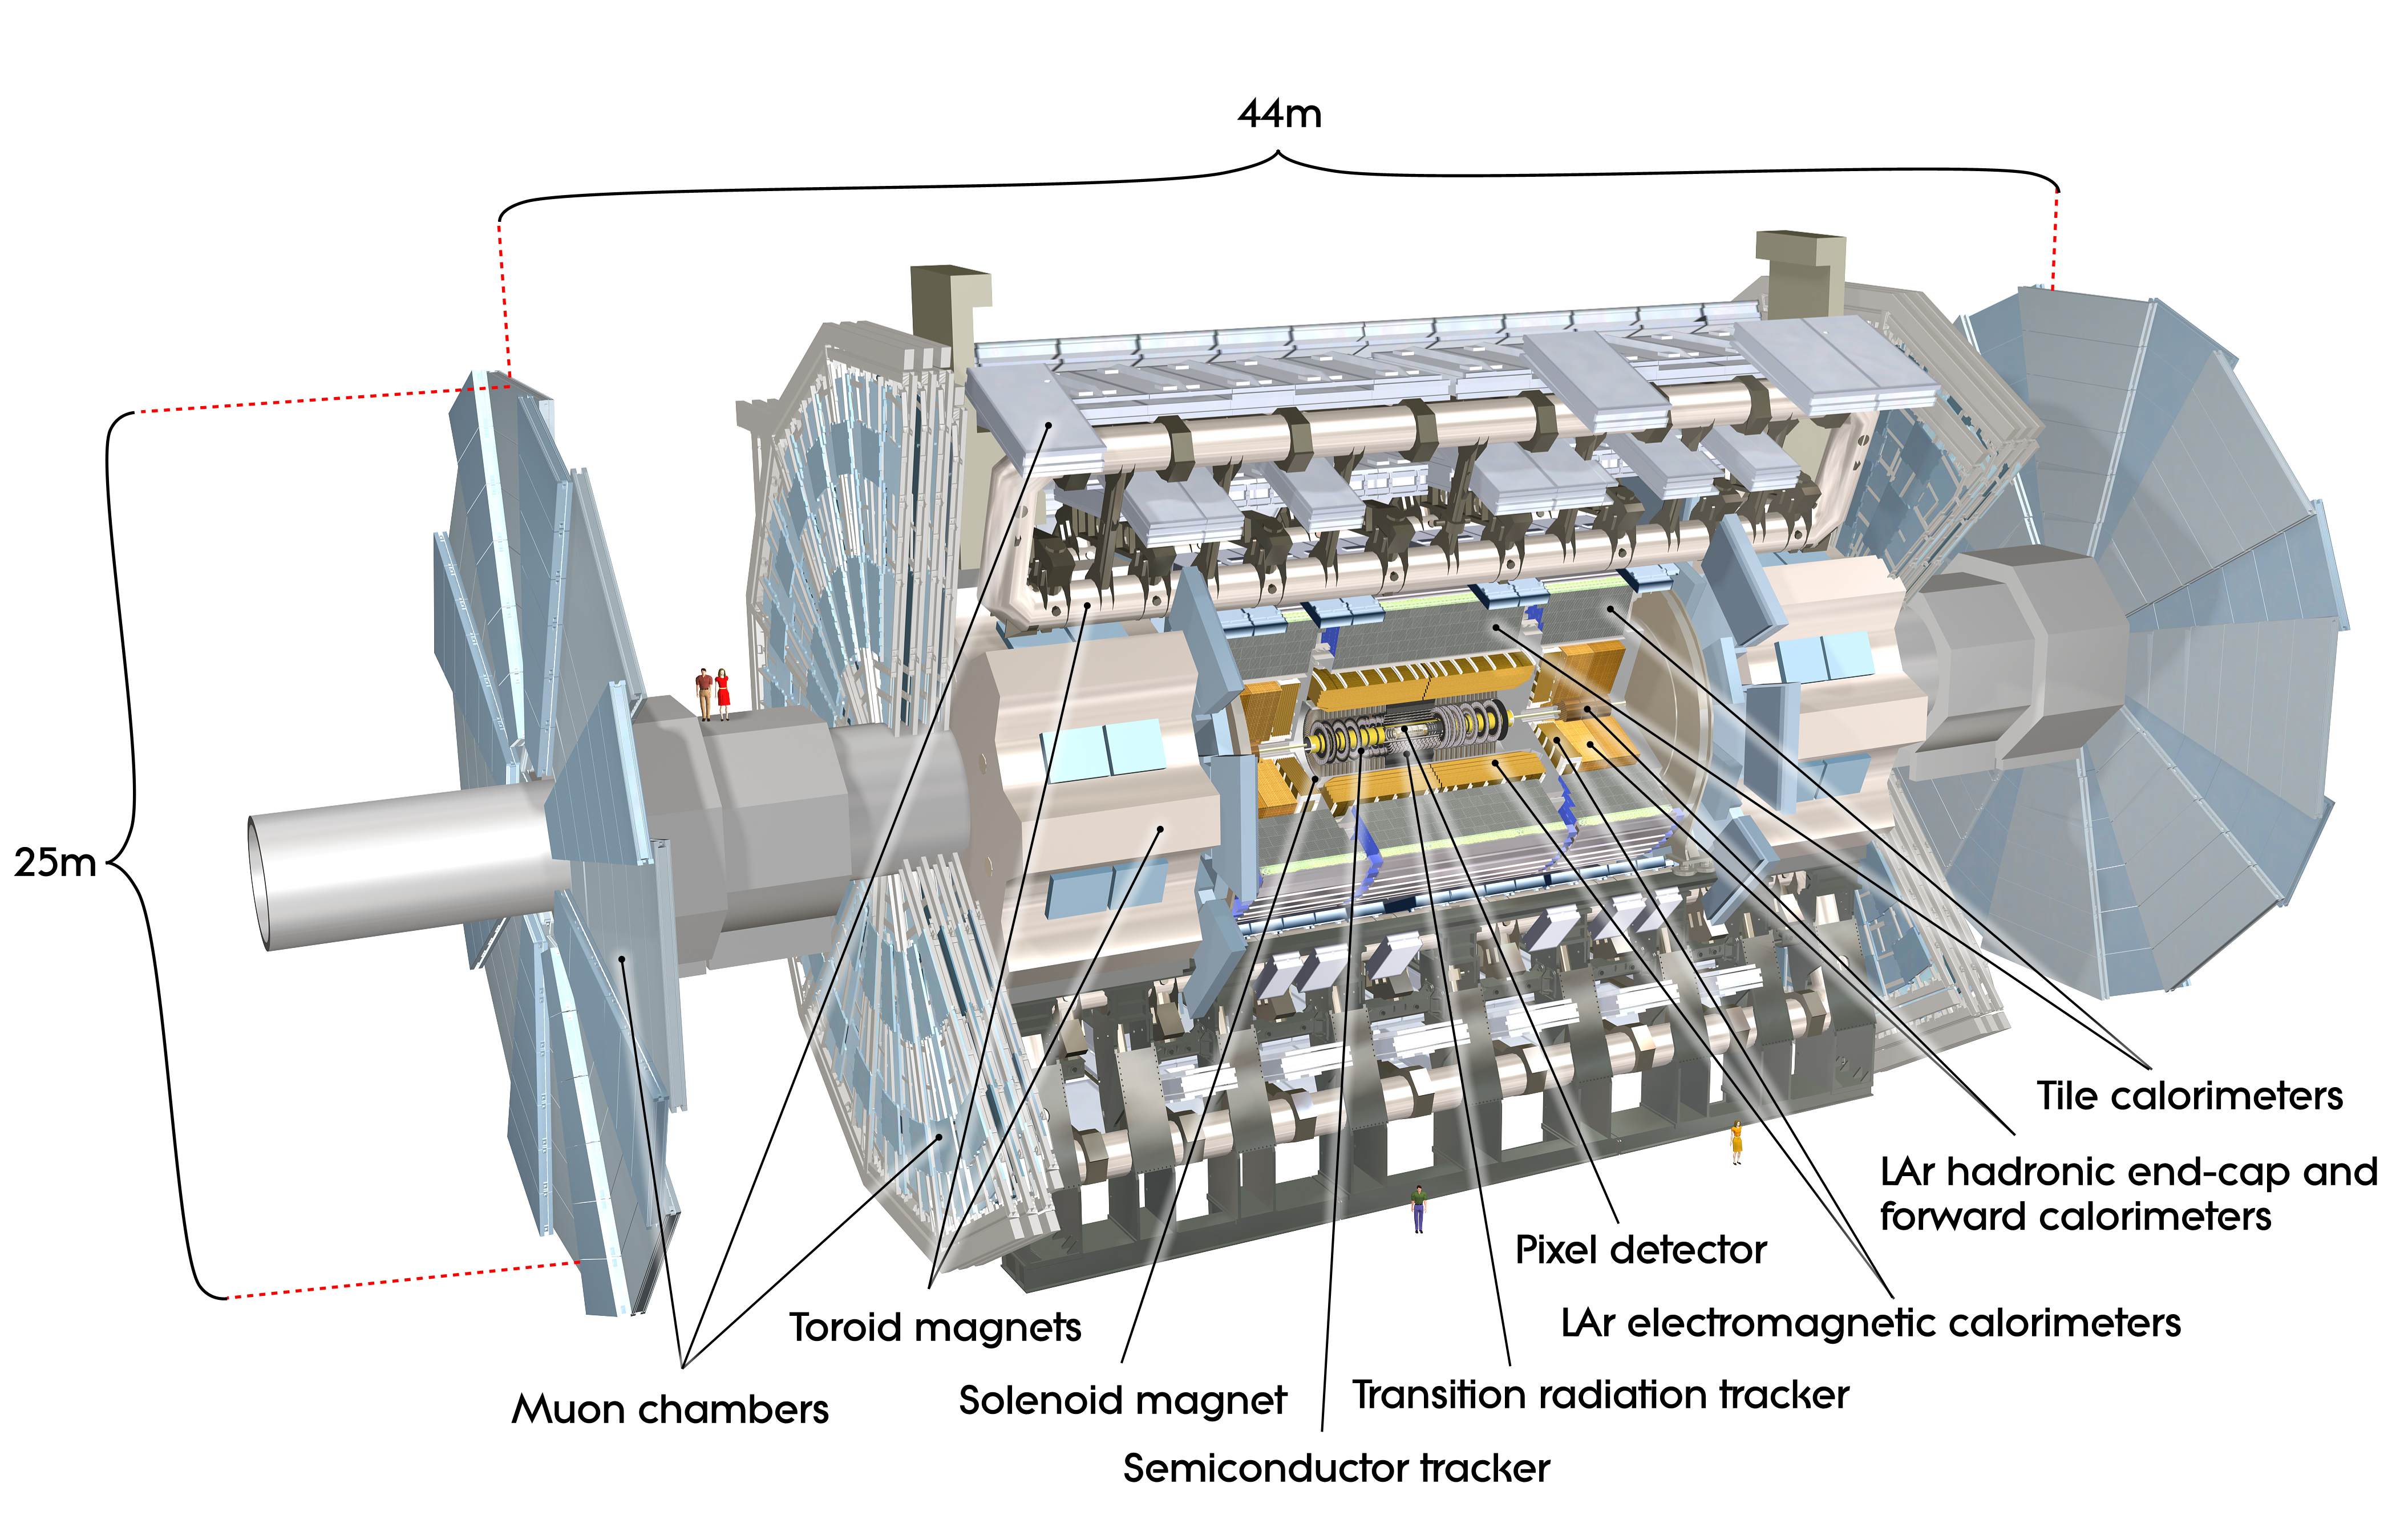
\includegraphics[clip,width=12cm]{fig/2/0803012_01.jpg}
  \caption{ATLAS検出器の全体図\cite{Aad:1129811}。直径 25 m、長さ 44 m の円筒型をしており、内部飛跡検出器、カロリーメータ、ミューオン検出器などの検出器を組み合わせて粒子の測定を行っている。}
  \label{fig:ATLAS検出器}
\end{figure}

\subsection{ATLAS検出器における座標系}
ATLAS実験では図~\ref{fig:a}に示すような直行座標系と円筒座標系が使用されている。直行座標系では、検出器の中心を原点として、ビーム軸に沿って$z$軸を取る。ビーム軸に垂直な平面を$x-y$平面としたときに、加速器の中心方向を正とする$x$軸及び、地面に対して垂直方向上向きを正とする$y$軸を設定する。円筒座標系では、ビーム軸に沿った$z$軸に対し、動径方向を$R$、ビーム軸周りの角度を方位角$\phi$、ビーム軸からの角度を極角$\theta$としている。
%ATLAS検出器ではz軸が正の側をA-side、負の側をC-sideと定義している。

また、ATLAS実験で使用される座標系として、
\begin{equation}
 \eta=-\ln\bigg(\tan\frac{\theta}{2}\bigg)
 \label{ラピディティ}
\end{equation}
と定義される擬ラピディティ$\eta$が用いられる。
ATLAS 検出器は円筒形をしており、$|\eta| < 1.0$ の側面部分をバレル領域、$|\eta| > 1.0$ の底面部分をエンドキャップ領域と呼ぶ。

\begin{figure}[tb]
  \centering
  \includegraphics[clip, width=11cm]{fig/2/atlas_coordinate_fix.pdf}
  \caption{ATLAS検出器における座標系。}
  \label{fig:a}
\end{figure}

\newpage
\subsection{マグネットシステム}\label{magnetic_filed}
ATLAS 実験では、荷電粒子の運動量測定のために超伝導磁石を用いて磁場をかけている。超伝導磁石は2種類あり、衝突点付近で発生した荷電粒子の運動量測定のために用いられるソレノイド磁石とミューオンの運動量測定のために用いられるトロイド磁石が設置されている。
図~\ref{fig:磁石}にATLAS検出器に設置されている超伝導磁石の配置を示す。
ソレノイド磁石は内部飛跡検出器とカロリメータの間に設置されており、この電磁石が作り出す磁場によって荷電粒子を曲げ、内部飛跡検出器でその曲率を測定することによって横方向運動量を測定する。
トロイド磁石によって生じる磁場の$\eta$分布を図~\ref{fig:磁場eta}に、$x-y$平面での磁場の分布を図~\ref{fig:磁場平面}に示す。
トロイド磁石はバレル部とエンドキャップ部に分けられ、それぞれ$\phi$方向に8つずつ等間隔で配置されてる。そのため、8回転対象の磁場構造を生み出しており、この磁場構造を考慮した上で様々な検出器が設置されている。

%ATLAS実験では、トロイド磁石が作り出す磁場によってミューオンを曲げることで、ミューオンの横方向運動量を測定する。


\begin{figure}[tb]
  \centering
  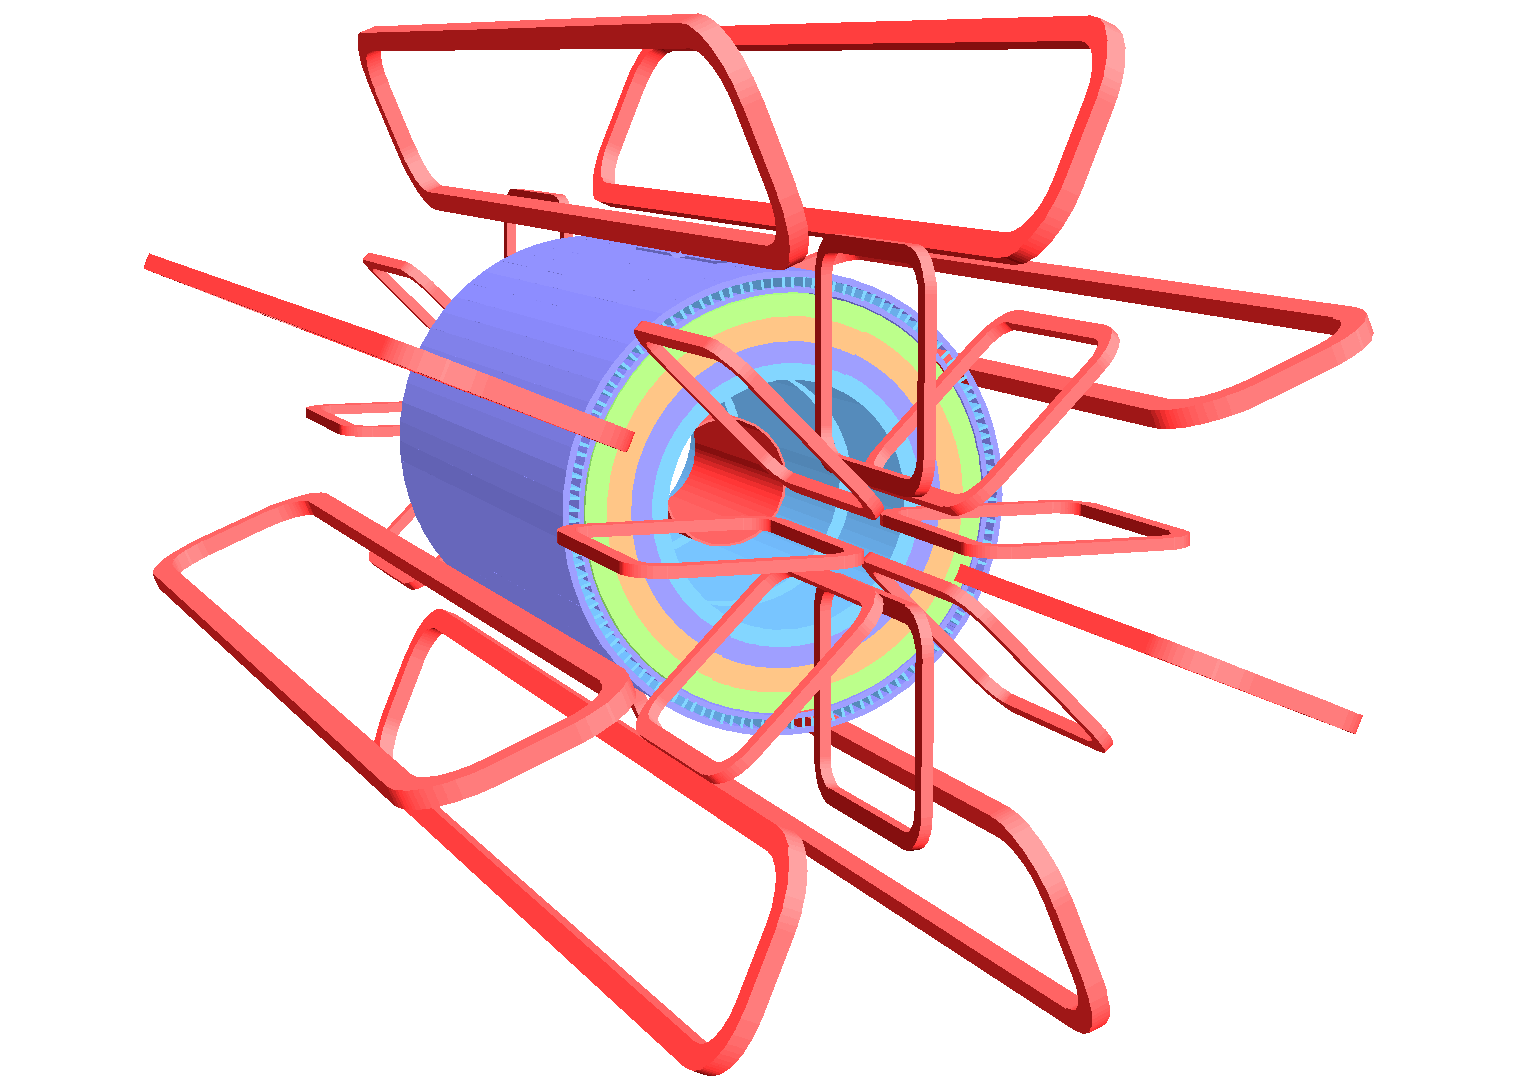
\includegraphics[clip, width=9cm]{fig/2/ATLcoilGeom.pdf}
  \caption{ATLAS検出器で用いられる超伝導磁石の配置\cite{Aad:1129811}。}
  \label{fig:磁石}
\end{figure}

\begin{figure}
    \centering
    \begin{minipage}[b]{0.5\linewidth}%
        \centering
        \hspace*{-1cm}
        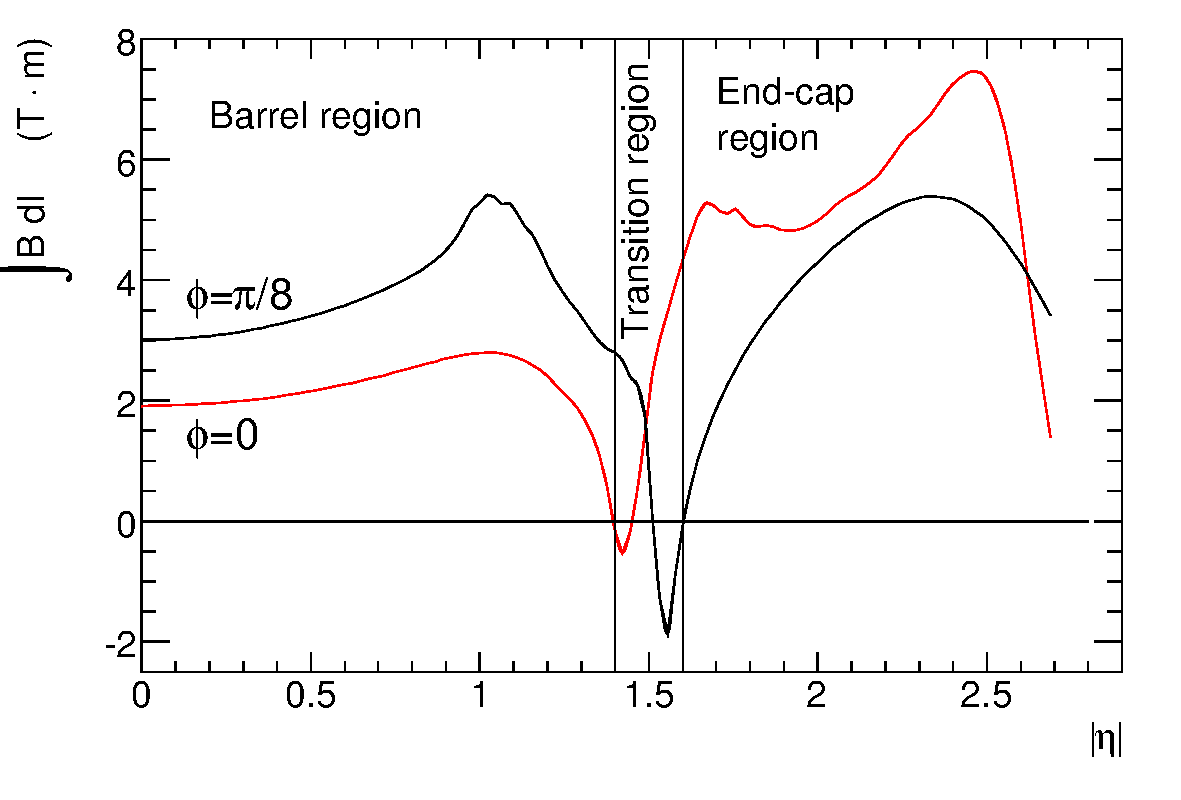
\includegraphics[clip, width=8cm]{fig/2/IBdl.pdf}
        \vspace{10pt}
        \subcaption{トロイド磁石による磁場の$\eta$分布\cite{Aad:1129811}。}
        \label{fig:磁場eta}
    \end{minipage}%
    %\hfill
    \begin{minipage}[b]{0.6\linewidth}%
        \centering
%\hspace*{1cm}
        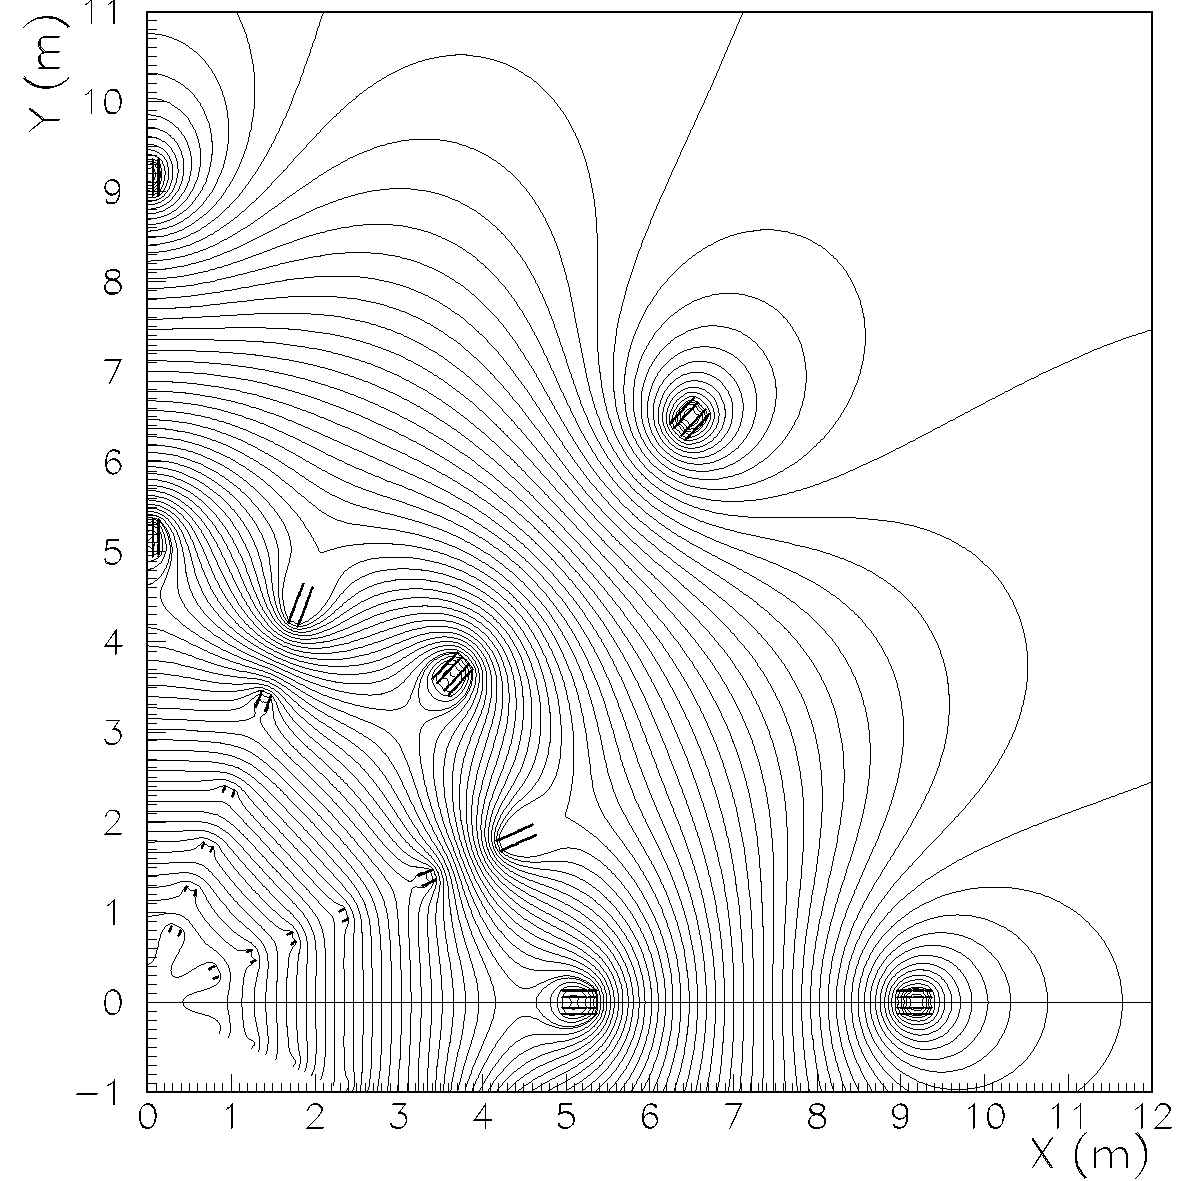
\includegraphics[clip, width=6cm]{fig/2/FMBmap.pdf}
        \vspace{10pt}
        \subcaption{ビーム軸から見た$x−y$平面での磁場の分布\cite{article:ATLASMagneticField}。}
        \label{fig:磁場平面}
    \end{minipage}%
    \caption{トロイド磁石の磁場の分布。設置位置の影響により磁場構造が一様ではない。}
    \label{fig:磁場}
\end{figure}




\subsection{内部飛跡検出器}
内部飛跡検出器はビーム衝突点に最も近い位置に設置され、衝突点で発生した荷電粒子の飛跡を測定する。内部飛跡検出器は内側からピクセル検出器~(Pixel)、Semiconductor Tracker~(SCT)、Transition Radiation Tracker~(TRT)で構成されている。
図~\ref{fig:内部飛跡検出器}に内部飛跡検出器の概略図を示す。

Pixelは最内層に設置された$|\eta| < 2.5$ の領域をカバーする半導体検出器であり、バレル部では同心円状に4層、エンドキャップ部ではディスク状のものが3層設置されている。位置分解能はバレル部で$R-\phi$平面で10~$\mu$m、$z$軸方向で115~$\mu$m、エンドキャップ部においては$R-\rm{\phi}$平面で10~$\mu$m、R方向で115~$\mu$mであり、高い位置分解能を持つ~\cite{Aad:1129811}。
SCTはPixelの外側に位置されており$|\eta| < 2.5$の領域をカバーしている。マイクロストリップと呼ばれる細長い有感領域をシリコン上に施した半導体検出器であり、バレル部ではビームパイプを中心とした同軸円筒状、エンドキャップ部ではビームパイプに垂
直なディスク状の検出器が設置されている。位置分解能はバレル部で$R-\phi$平面で17~$\mu$m、$z$軸方向で580~$\mu$m、エンドキャップ部においては$R-\phi$平面で17~$\mu$m、$R$方向で580~$\mu$mである\cite{Aad:1129811}。
TRTは内部飛跡検出器の最外層に位置する検出器であり、飛跡のトラッキングのほかに遷移輻射を利用した電子の同定も行っている。直径4~mmのドリフトチューブをバレル部では73層、エンドキャップ部では160層に積み重ねることで構成されている。ドリフトチューブはバレル部ではビーム軸方向に、エンドキャップ部では放射状に並べられている。1つのドリフトチューブの位置分解能は$R-\phi$平面で130~$\mu$m である。

また、横方向運動量に対する分解能は式~\eqref{equ:pt分解能}で表される~\cite{Aad:1129811}。
\begin{equation}
    \frac{\sigma_{p_{T}}}{p_{T}} = 0.05\times p_{T}\oplus 0.7 
 \label{equ:pt分解能}
\end{equation}
第1項は電子数をエネルギーに換算する際の統計的な揺らぎにの項であり、第2項はエネルギー較正の精度や温度の揺らぎによる項である。

\begin{figure}
    \centering
    \begin{minipage}[b]{0.4\linewidth}
        \centering
        \hspace*{-1cm}
        \includegraphics[clip, width=8cm]{fig/2/inner_detectoer1.jpg}
        \vspace{10pt}
        \subcaption{}
        \label{fig:内部飛跡検出器の概略図1}
    \end{minipage}
    \hfill
    \begin{minipage}[b]{0.5\linewidth}
        \centering
        \includegraphics[clip, width=7cm]{fig/2/inner_detector2.jpg}
        \vspace{10pt}
        \subcaption{}
        \label{fig:内部飛跡検出器の概略図2}
    \end{minipage}
    \caption{内部飛跡検出器の全体像及び断面図。(a): 全体像\cite{Aad:1129811}、(b): バレル部の断面図\cite{Collaboration:2723878}。内側から順に Pixel, SCT, TRT 検出器が設置されている。}
    \label{fig:内部飛跡検出器}
\end{figure}



\subsection{カロリメータ}
カロリメータは内部飛跡検出器の外側に設置されており、内側から電磁カロリメータ、ハドロンカロリメータの順に配置されている。電磁カロリメータは電磁シャワーを用いて電子と光子のエネルギーや位置を測定し、ハドロンカロリメータは強い相互作用によるハドロンシャワーを用いてハドロンのエネルギーやそれを組み合わせたジェットのエネルギーを測定する。
図~\ref{fig:カロリメータ}にATLAS検出器で用いられるカロリメータの概略図を示す。

\begin{figure}[tb]
  \centering
  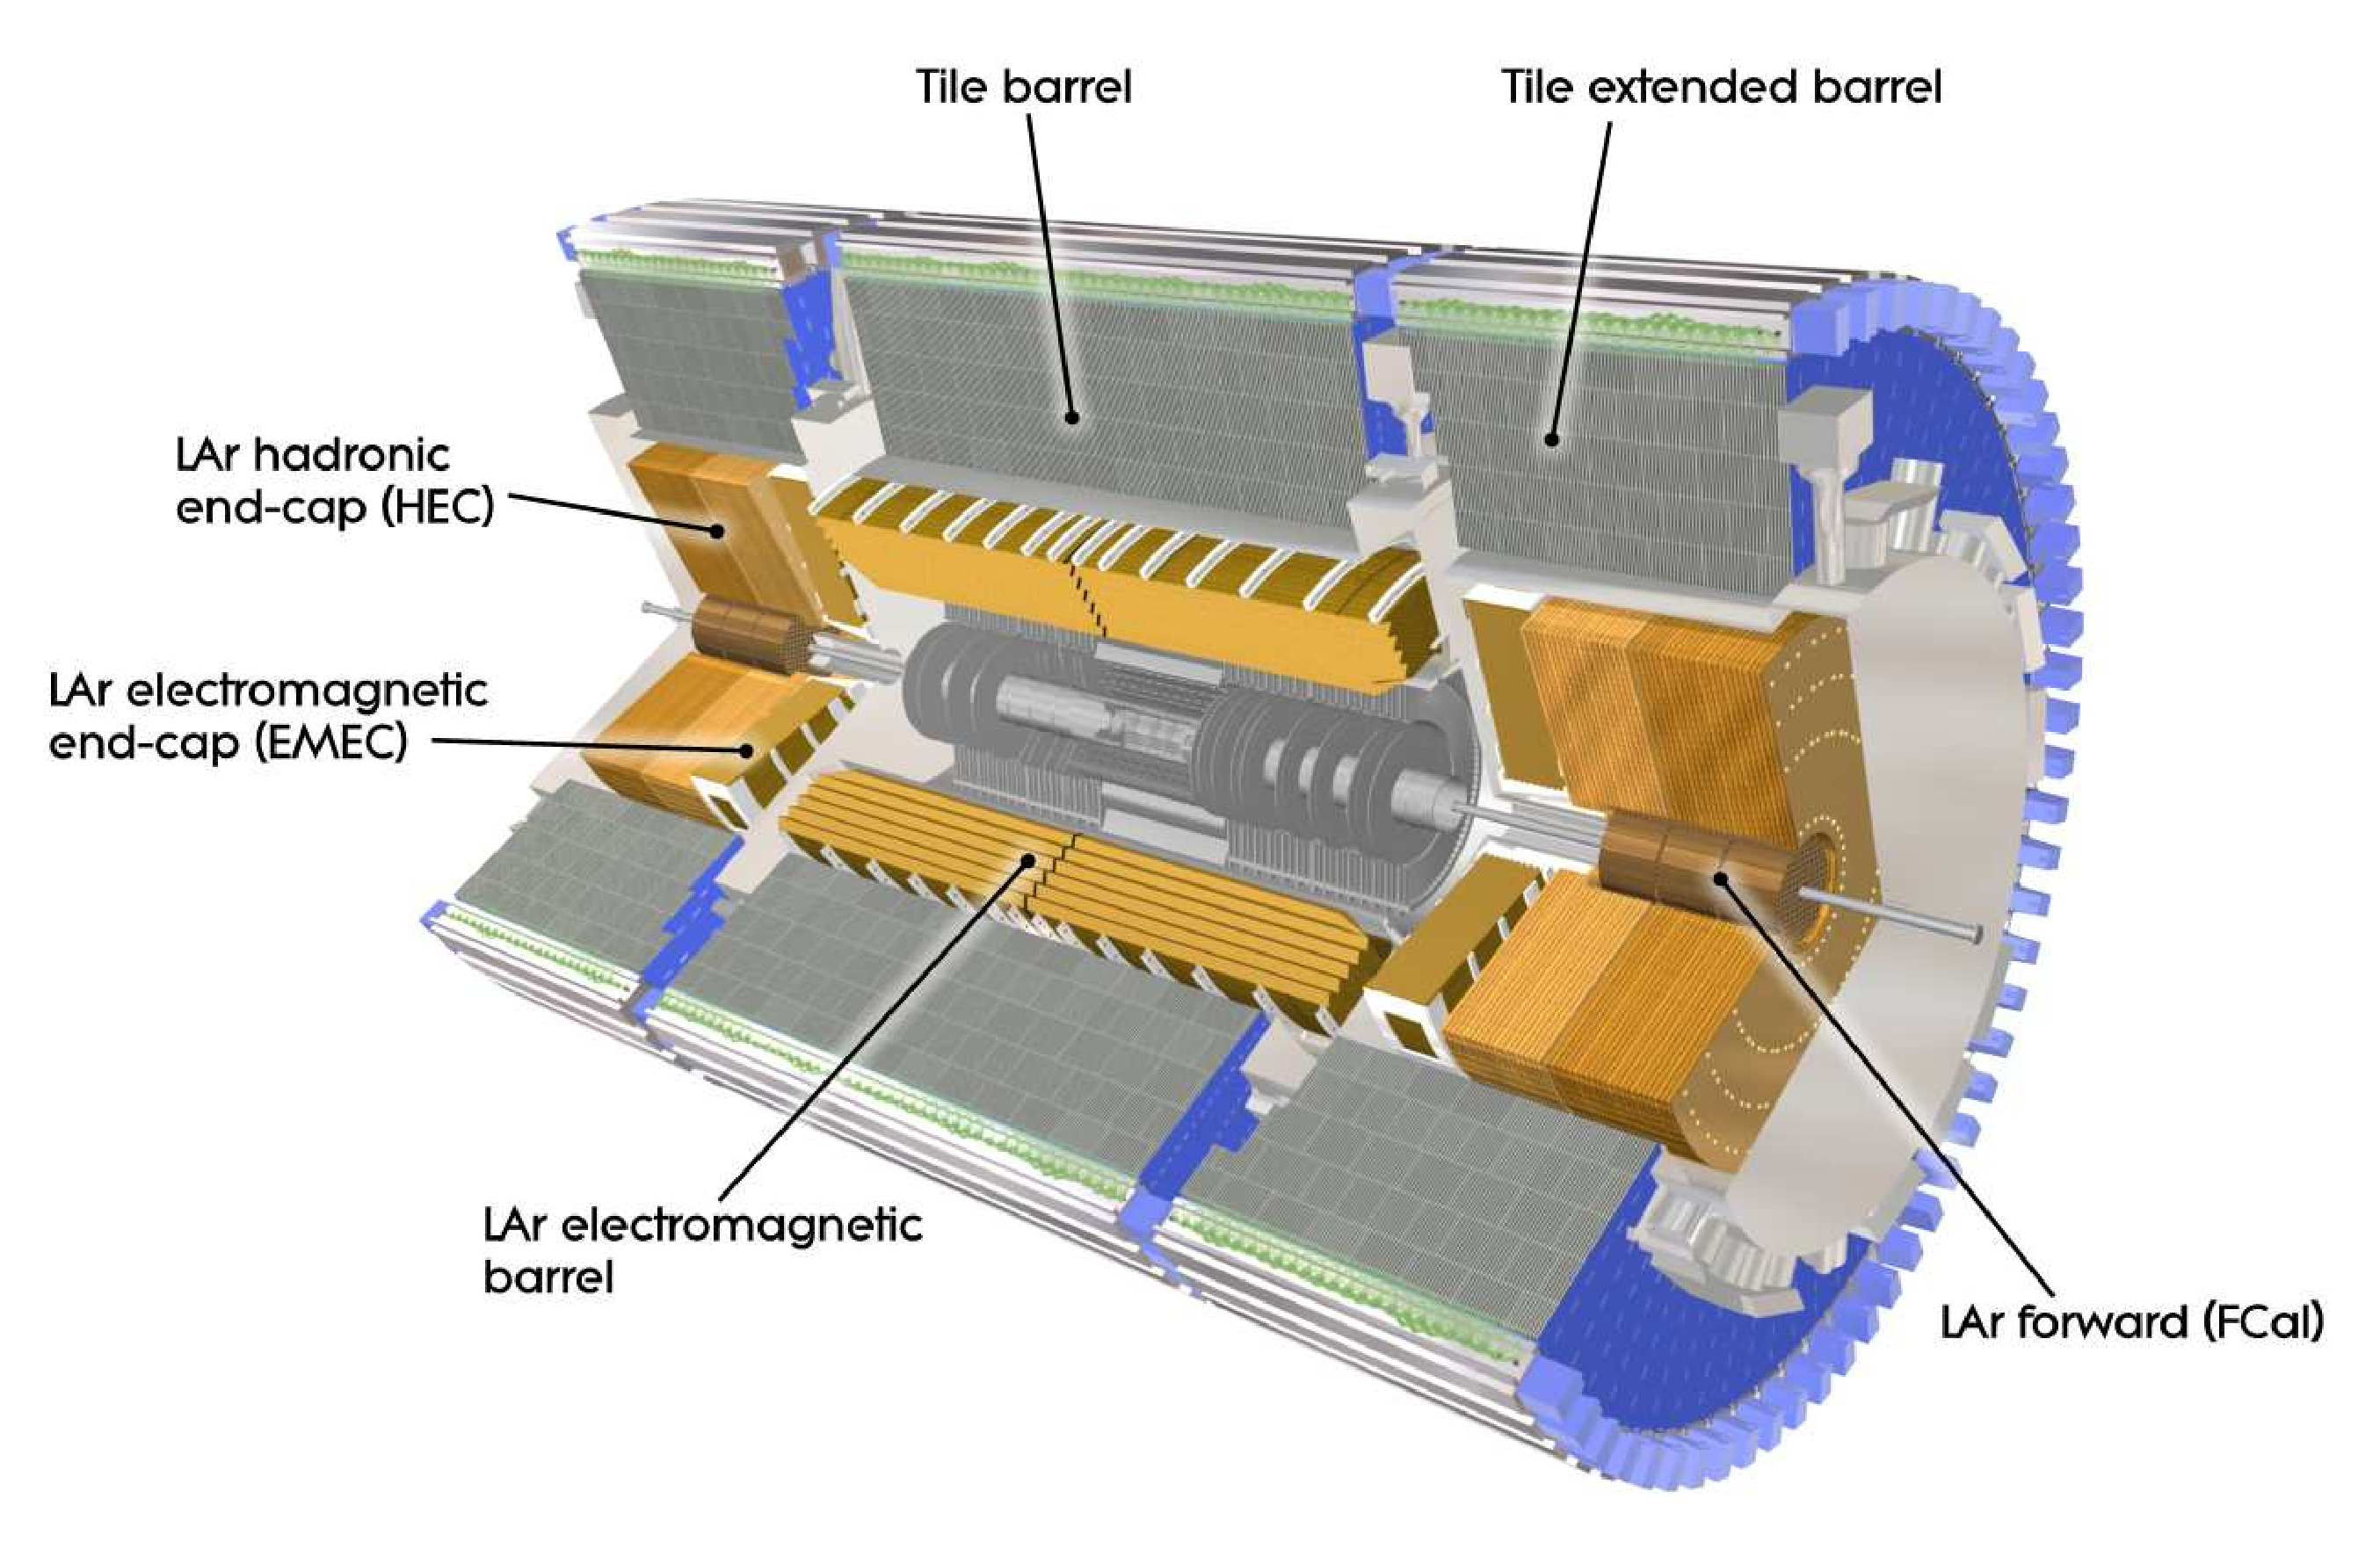
\includegraphics[clip, width=11cm]{fig/2/Calorimeter_d3.pdf}
  \caption{ATLAS 検出器におけるカロリメータの構成~\cite{Aad:1129811}。電磁カロリメータは、バレル領域およびエンドキャップ領域の 2 種類。ハドロンカロリメータは、バレル領域のタイル、エンドキャップ領域、フォワード領域の液体アルゴンカロリメータの3種類。}
  \label{fig:カロリメータ}
\end{figure}

\subsubsection{電磁カロリメータ}
電磁カロリメータでは、電磁相互作用をする粒子である電子及び光子の同定、それらのエネルギーを精密に測定する。
ATLAS検出器には、$|\eta|<1.5$にバレル部をカバーするバレルカロリメータ、$1.4<|\eta|<3.4$の両側のエンドキャップ部をカバーするエンドキャプカロリメータが設置されている。
バレル部とエンドキャプ部ともに、吸収層の鉛と検出層の液体アルゴンで構成されたカロリメータであり、電磁相互作用を起こす光子や電子のエネルギーと位置を測定する役割を担っている。

また、エネルギー分解能$\sigma_{E}$は式~\eqref{equ:電子エネルギー分解能}のように表される~\cite{Aad:1129811}。
\begin{equation}
    \frac{\sigma_{E}}{E} = \frac{10}{\sqrt{E}}\oplus 0.7
 \label{equ:電子エネルギー分解能}
\end{equation}



\subsubsection{ハドロンカロリメータ}
ハドロンカロリメータは電磁カロリメータの外側に設置されており、タイルカロリーメータ、エンドキャップカロリーメータ、フォワードカロリーメータの3つに分類され、それぞれ異なる$\eta$の範囲をカバーする。バレル部では、鉄の吸収体とタイル状のシンチレータから構成されたタイルカロリメータが設置されている。$1.5 < |\eta| < 3.2$のエンドキャプ部では、銅の吸収体と液体アルゴンから構成されたエンドキャプカロリメータが使用されている。さらに、$3.1 < |\eta| < 4.9$フォワード領域では銅とタングステンの吸収体と液体アルゴンからなるフォワードカロリメータが設置されている。

また、式~\eqref{equ:ハドロンエネルギー分解能バレル}にバレル部、式~\eqref{equ:ハドロンエネルギー分解能エンド}にエンドキャップ部の単一のハドロン粒子に対するエネルギー分解能を示す~\cite{Aad:1129811}。
\begin{equation}
    \frac{\sigma_{E}}{E} = \frac{52.3}{\sqrt{E}}\oplus 1.7 (バレル部)
 \label{equ:ハドロンエネルギー分解能バレル}
\end{equation}

\begin{equation}
    \frac{\sigma_{E}}{E} = \frac{62.4}{\sqrt{E}}\oplus 3.6 (エンドキャップ部)
 \label{equ:ハドロンエネルギー分解能エンド}
\end{equation}

\subsection{ミューオン検出器}\label{section2-2-4}
ミューオン検出器はATLAS検出器の最外層に設置されており、カロリメータを通過したミューオンを検出するために用いられおり、Resistive Plate Chamber~(RPC)とThin Gap Chamber~(TGC) という2種類のトリガー検出器と、Monitored Drift Tube~(MDT)の精密測定用の検出器によって構成される。Run-3からは磁場領域より内側にNew Small Wheel~(NSW)という検出器が新たに設置された。
図~\ref{fig:ミューオン検出器}にミューオン検出器の配置図を示す。

ミューオン検出器では、検出器を層状にまとめたステーションと呼ばれる単位で構成されており、エンドキャップ部ではビーム軸に対して垂直に円盤状のステーションを、バレル部では筒状のステーションによって構成されている。
これらのステーションはエンドキャップ部、バレル部それぞれ3つずつ設置されており、衝突点に近い方から Inner~(I), Middle~(M), Outer~(O)と呼ぶ。
また、図~\ref{fig:ミューオン検出器_エンド}と図~\ref{fig:ミューオン検出器_バレル部}に示すように、ミューオン検出器はトロイド磁石と干渉しないように配置するため、$\phi$方向においてはLarge Sector~(L)とSmall Sector~(S)の2種類の検出器を組み合わせてステーションを構成している。そのため、ミューオン検出器も磁石と同じく8回転対象になるように配置されている。


\begin{figure}[tb]
  \centering
  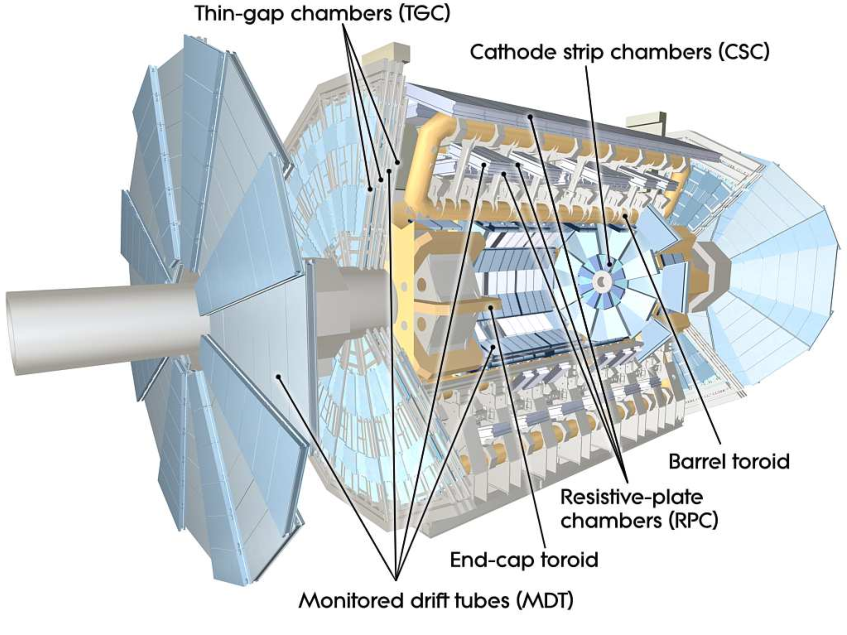
\includegraphics[clip, width=12cm]{fig/2/muondetector.pdf}
  \caption{ミューオン検出器の配置図\cite{Aad:1129811}。バレル部には RPC、MDT、エンドキャップ部には TGC、MDT、CSC が配置されている。}
  \label{fig:ミューオン検出器}
\end{figure}

\begin{figure}[p]
    %\centering
    %\begin{tabular}{c}
    \vspace{-100pt}
    \begin{minipage}[t]{\hsize}
        %\centering
        \hspace*{1cm}
        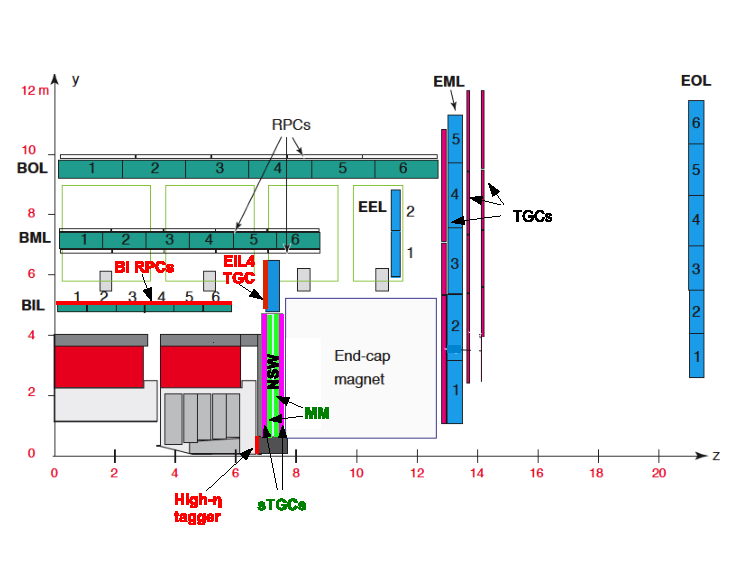
\includegraphics[clip, width=12cm]{fig/2/muon_Rz_Large.pdf}
        %\vspace{5pt}
        \subcaption{Large Sectorでのミューオン検出器の配置図}
        %\label{}
    \end{minipage}\\
    %\hfill
    
    \begin{minipage}[b]{\hsize}
        %\centering
        \hspace*{1cm}
        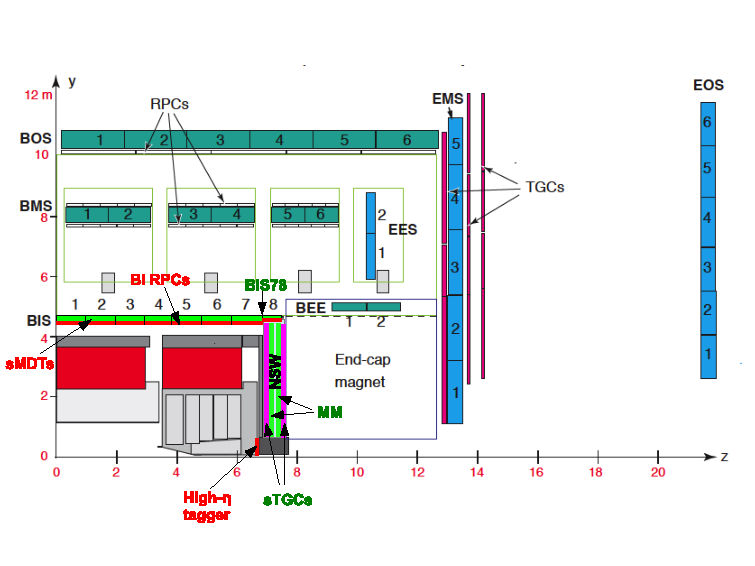
\includegraphics[clip, width=12cm]{fig/2/muon_Rz_small.pdf}
        %\vspace{5pt}
        \subcaption{Small Sectorでのミューオン検出器の配置図}
        \label{fig:検出器_エンド}
    \end{minipage}
    %\end{tabular}
    \caption{$R-x$方向からみたミューオン検出器の配置図\cite{article:phase2}~ Large Sector と Small Sector では、トロイド磁石の配置の関係で磁場領域より内側にある検出器の配置が大きく異なる。}
    \label{fig:ミューオン検出器_エンド}
\end{figure}

\begin{figure}[tb]
  \centering
  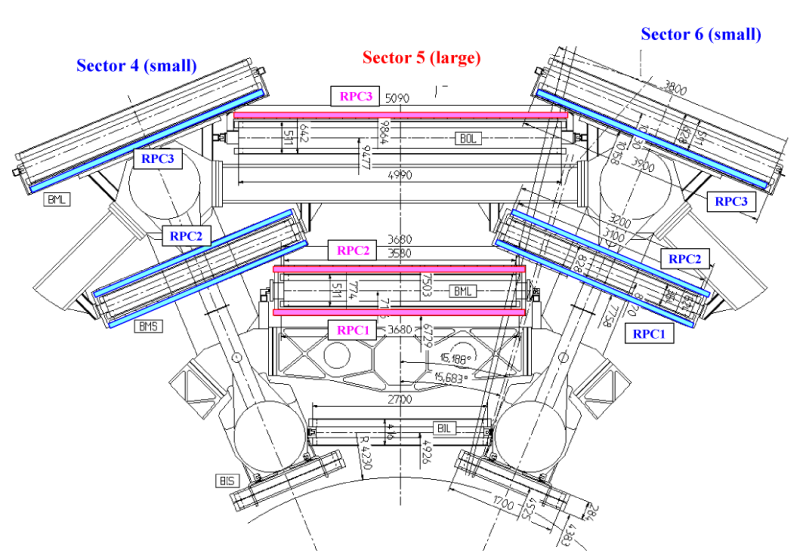
\includegraphics[clip, width=12cm]{fig/2/RPC_xy.pdf}
  \caption{ビーム軸から見たバレル部のミューオン検出器の配置図\cite{Aad:1129811}。トロイド磁石および支持構造に干渉しないように、Large SectorとSmall Sectorを組み合わせて設置されている。}
  \label{fig:ミューオン検出器_バレル部}
\end{figure}


\subsubsection{Resisitive Plate Chamber (RPC)}
RPCは$|\eta| < 1.05$のバレル部のミューオントリガー判定に用いられる平行電極板のガス検出器である。図~\ref{fig:RPC} にRPC検出器の構造を示す。2枚の高抵抗プレートの間に幅2~mmの絶縁体を挟み込んでおり、プレート間のには約4.9~kV/mmの電場が形成されている。電場に沿ってガスから電離した電子が雪崩増幅を起こし、プレートの外面に取り付けられたストリップで信号を読み取り、直交するストリップの情報から$\eta$と$\phi$の位置を導出する。RPCの位置分解能は$z$方向に10~mm、$\phi$方向に10~mmである。

\begin{figure}[tb]
  \centering
  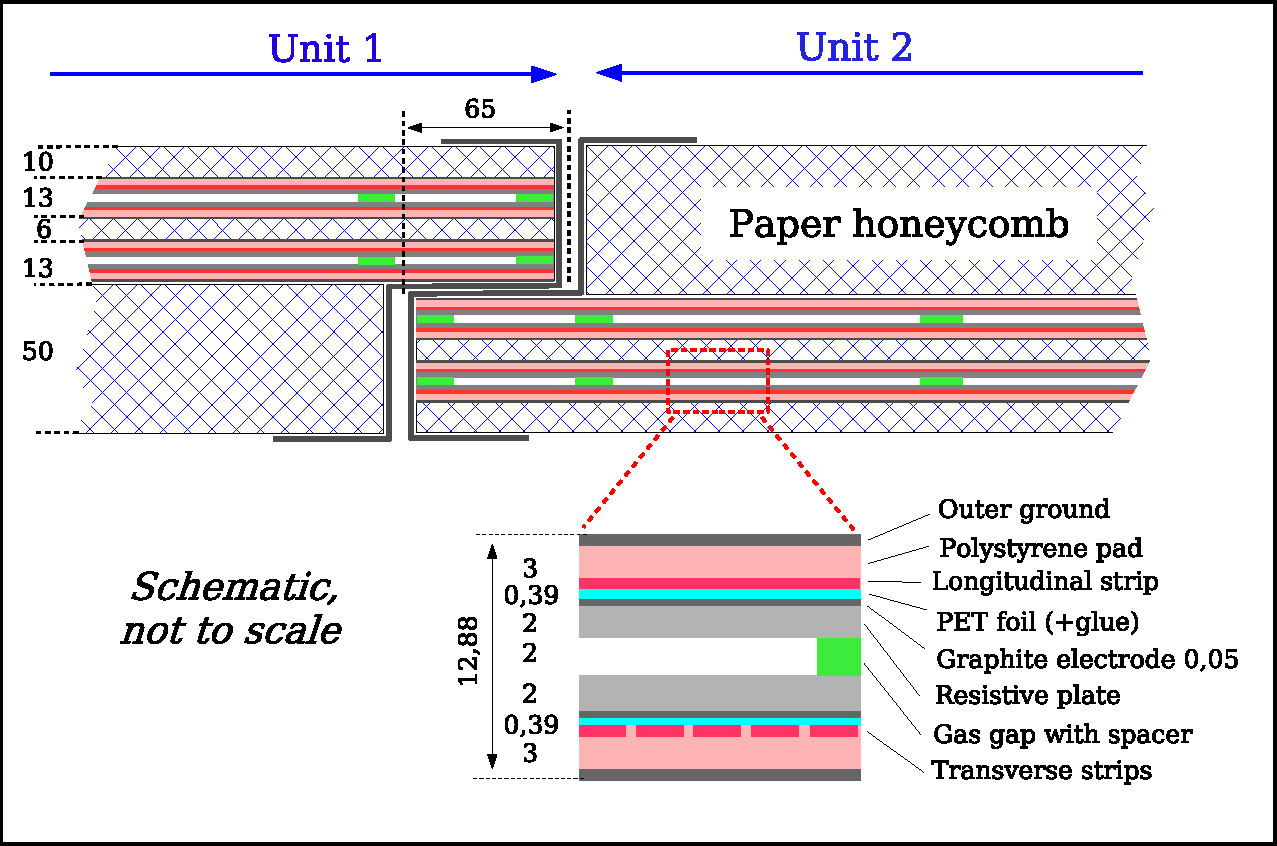
\includegraphics[clip, width=10cm]{fig/2/RPC_structure.pdf}
  \caption{RPCの構造\cite{Aad:1129811}}
  \label{fig:RPC}
\end{figure}

図~\ref{fig:検出器_エンド}に示すBISはBarrel Inner Small sectorの略であり、RPCの最内層に設置された検出器である。RPCの最内層の検出器は$z$軸に沿って1から8までナンバリングされており、その7番目と8番目の位置の検出器はRun-3から新たに導入された検出器である。このRPC~BIS78は$1.0 < |\eta| < 1.3$における領域をカバーしており、\ref{innnercoin}節で述べるインナーコインシデンスの際に重要な役目を果たす。

\subsubsection{Thin Gap Chambers (TGC)}
TGCはエンドキャプ部の$1.05 < |\eta| < 2.7$の領域に設置されているミューオン検出器である。図~\ref{fig:TGC_st}にTGC検出器の配置図を示す。
TGCはMulti Wire Proportional Chamber~(MWPC)の一種で、ワイヤーとストリップによる2次元読み出しを行うことでミューオンのヒット位置を測定する。図~\ref{fig:MWPC}にTGCの構造を示す。
アノードワイヤーには直径50~$\mu$mの金メッキをしたタングステンワイヤーを用い、カソードには片面に表面抵抗1~M$\Omega$のカーボンを塗布したガラスエポキシ板を用いている。反対側の面には銅で出来たストリップがワイヤーに直交するように張られている。ミューオンの位置情報のうち$R$をアノードワイヤーで、$\phi$をカソードストリップで測定することで2次元での読み出しが可能となっており、TGCの分解能は$R$方向に2$\sim$6~mm、$\phi$方向に3$\sim$7~mmである。

図~\ref{fig:TGC}に示すように、TGCを構成する検出器には2層構造のDoubletと3層構造のTripletの2種類がある。
Doubletはワイヤー面2層とストリップ面2層から信号の読み出しを行う。Tripletは3層構造になっているが、真ん中の層にストリップ面はないためワイヤー面3層とストリップ面2層から信号の読み出しを行う。

図~\ref{fig:TGC_st}に示すようにTGC検出器はトロイド磁石による磁場領域より内側にEI~(Endcap Inner), FI~(Forward Inner)と呼ばれる2つのステーション、磁場領域より外側にM1, M2, M3~(Middle~1, Middle~2, Middle~3)と呼ばれる3つのサブステーションが配置されており、M1, M2, M3の3つのステーションを合わせてTGC Big Wheel~(TGC BW)と呼ぶ。M1はTriplet構造であり、EI/FI、及びM2、M3はDoublet構造である。
M1, M2, M3は図~\ref{fig:TGC_oc}のように複数のチェンバーを組み合わせた円盤状の検出器である。
%$1.05 < |\eta| < 1.92$ の領域をエンドキャップ領域、$1.92 < |\eta| < 2.4$ の領域をフォワード領域と呼ぶ。

\begin{figure}[tbp]
  \centering
  \vspace{50pt}
  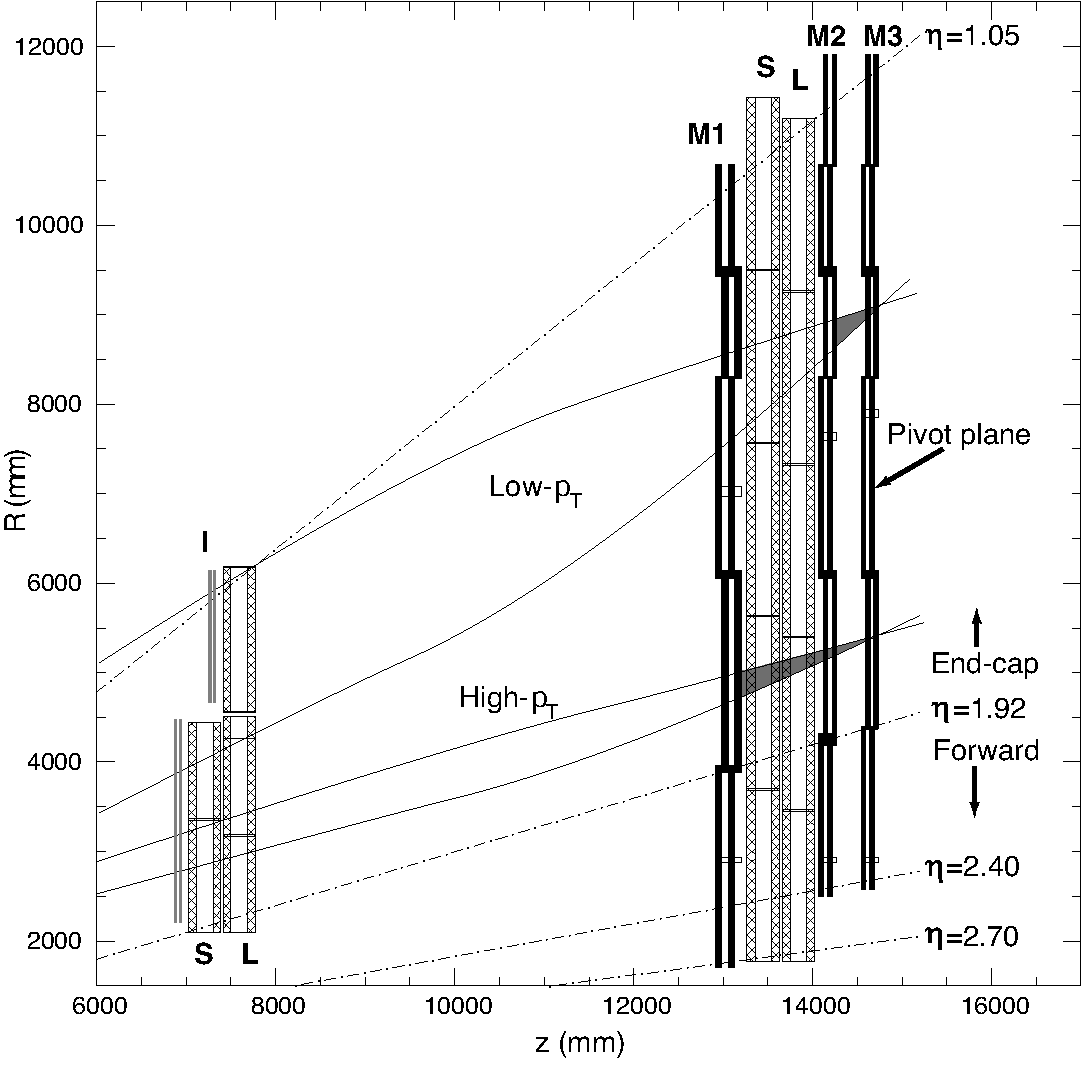
\includegraphics[clip, width=14cm]{fig/2/l1mue-schema.pdf}
  \caption{TGC検出器の配置図~\cite{Aad:1129811}。磁場領域の内側にEI、FI、外側にTGC-BWと呼ばれる3層のステーション(M1, M2, M3)が設置されている。Run-3では内側のEI, FIに代わり、NSWが設置されている。}
  \label{fig:TGC_st}
\end{figure}


\begin{figure}[tb]
  \centering
    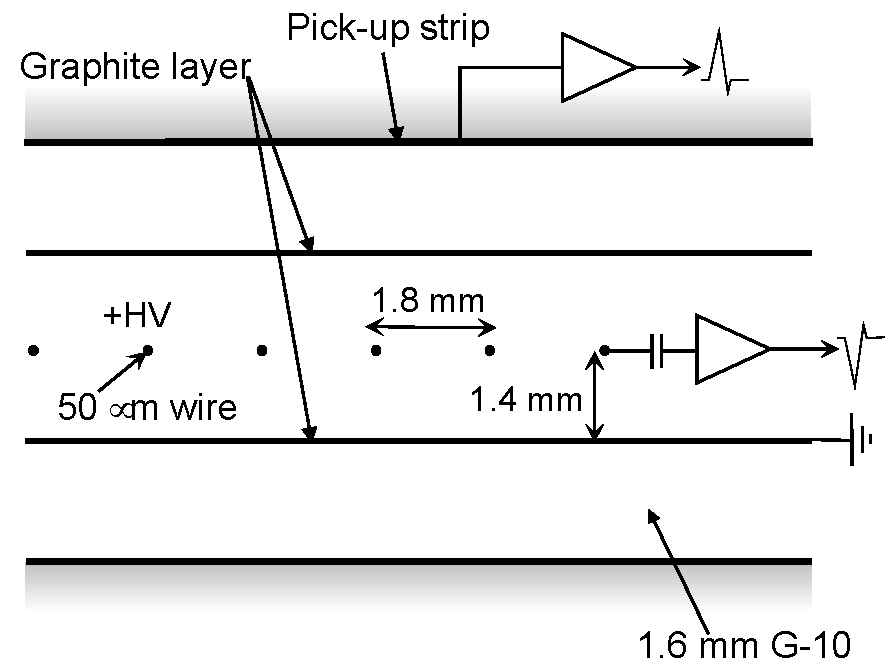
\includegraphics[clip, width=8cm]{fig/2/TGC_anode_wire.pdf}
  \caption{TGC 検出器の構造\cite{Aad:1129811}。ガスギャップ2.8~mm、ワイヤー間隔2.8~mmのMWPC~(Multi
Wired Proportional Chamber)の構造をしている。}
  \label{fig:MWPC}
\end{figure}

\begin{figure}[tb]
  \centering
  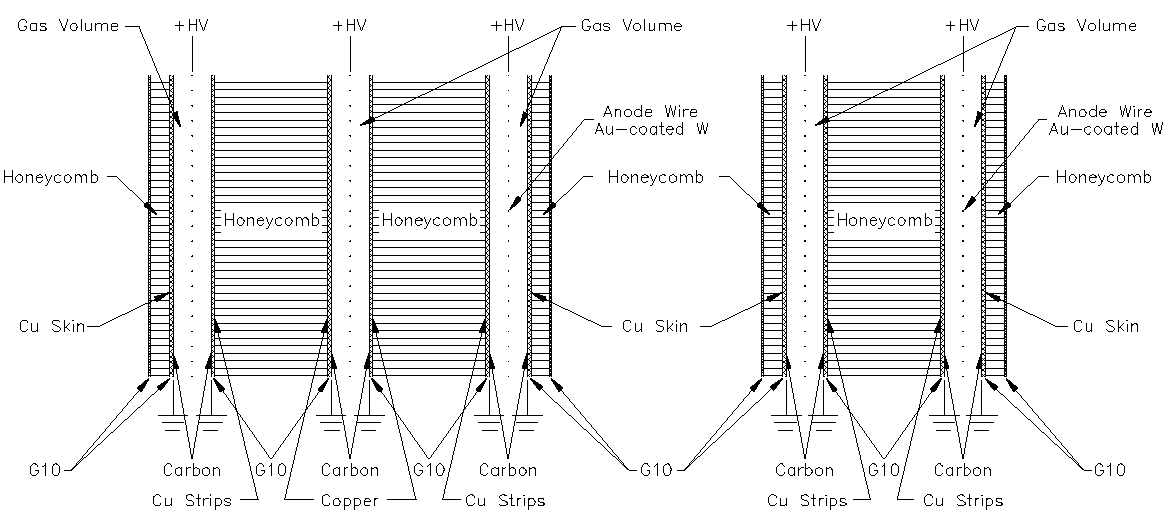
\includegraphics[clip, width=13cm]{fig/2/TGC_construction.pdf}
  \caption{TGC Triplet と Doublet の断面図\cite{Aad:1129811}。}
  \label{fig:TGC}
\end{figure}

\begin{figure}[tb]
  \centering
  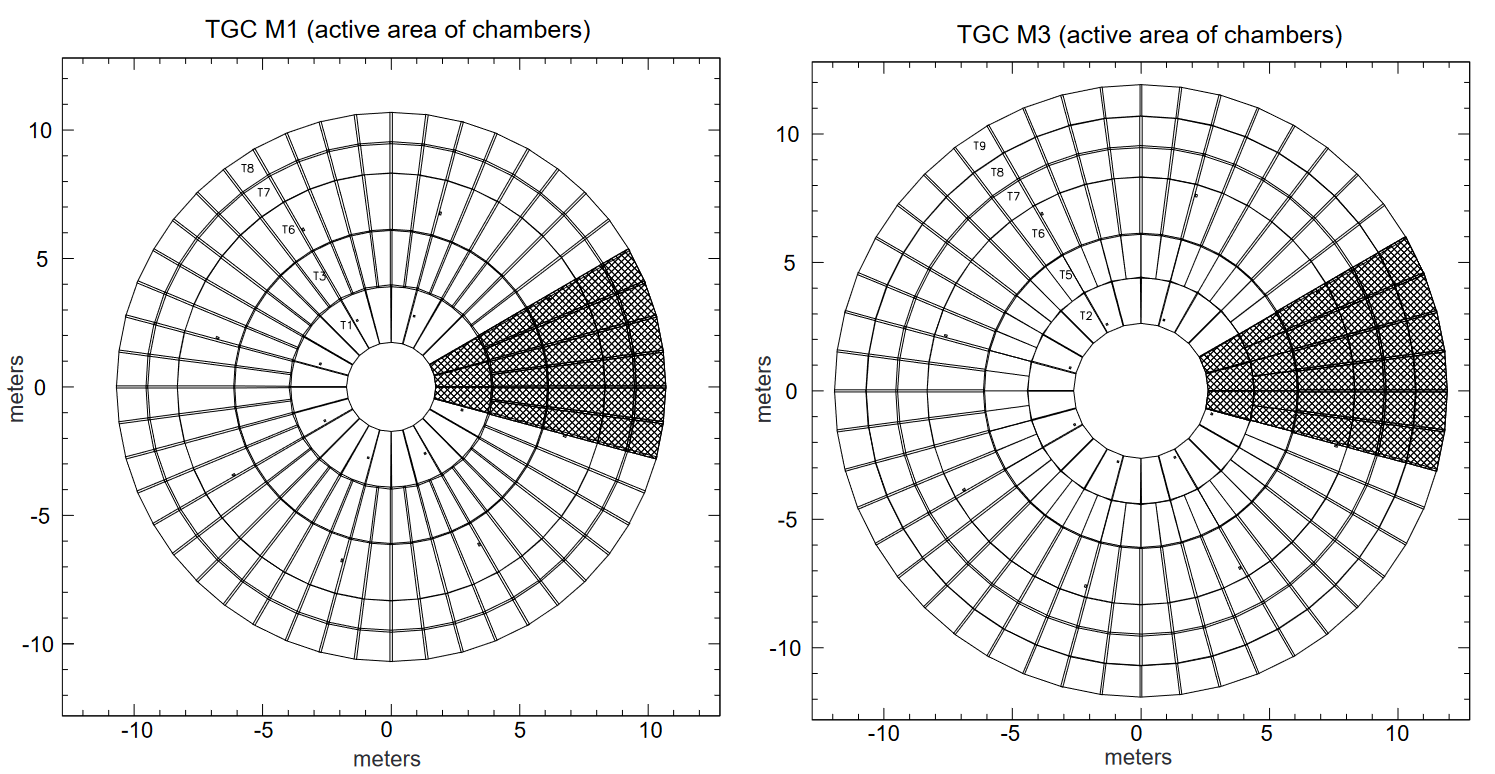
\includegraphics[clip, width=14cm]{fig/2/TGC_octant.png}
  \caption{TGC 検出器 の M1,M3 ステーションの概要図\cite{Lellouch:684103}。実線で囲まれたマスが 1 つのチェンバーに対応する。}
  \label{fig:TGC_oc}
\end{figure}

\subsubsection{Monitored Drift Tube (MDT)}
MDT はミューオンの飛跡の精密測定を目的とした検出器であり、直径約30~mmのドリフトチューブを6層または8層並べた構造をしている。MDTの構造図を図~\ref{fig:MDT} に示す。ドリフトチューブには Ar/$\rm{CO_2}$ を封入している。電離によって生じた電子は、ドリフトチューブの中心に張られている直径50~$\rm{\mu}$m のアノードワイヤーで集められ、読み出される。MDTの位置分解能は35~$\mu$mである。

\begin{figure}[tb]
  \centering
  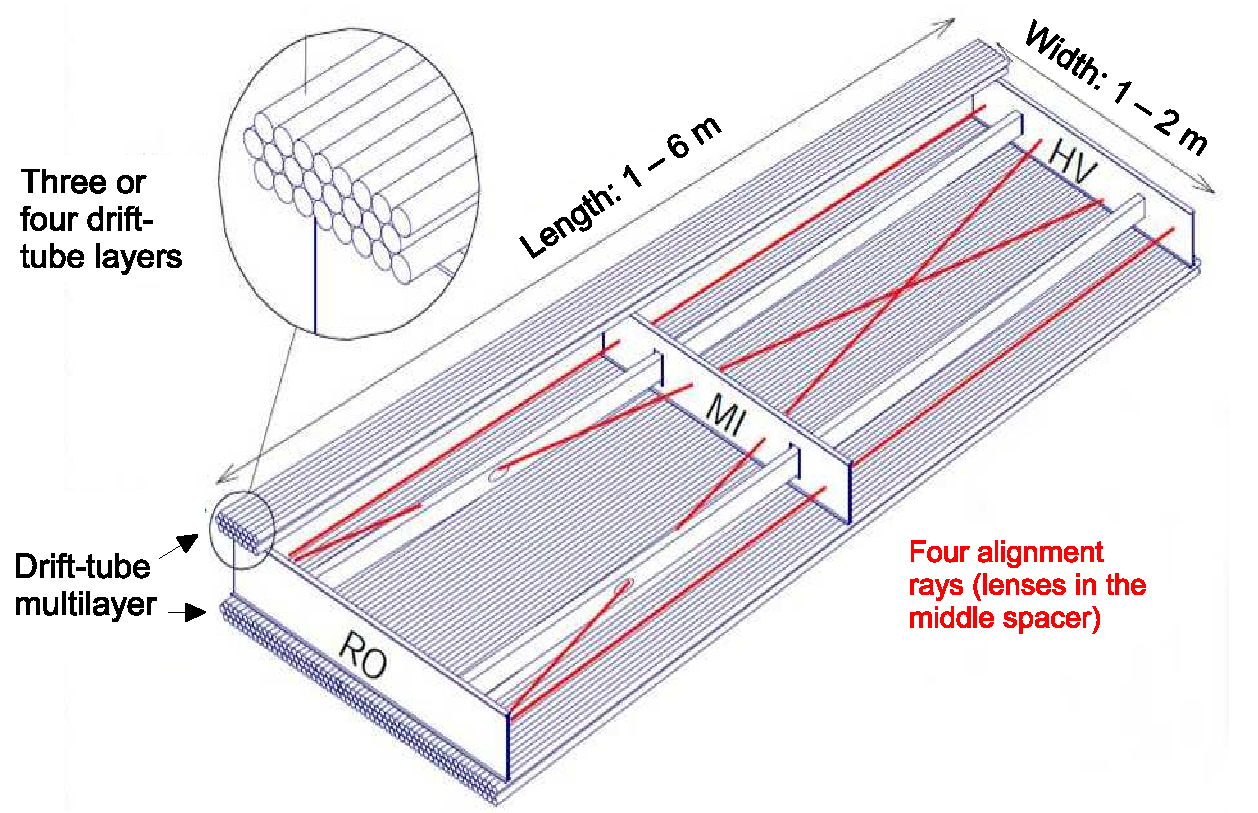
\includegraphics[clip, width=11cm]{fig/2/MDT_chamber_schematics_2.pdf}
  \caption{MDT の構造図\cite{Aad:1129811}。ドリフトチューブを積み重ねたような構造となっている。}
  \label{fig:MDT}
\end{figure}


\subsubsection{New Small Wheel (NSW)}
New Small Wheel~(NSW) は高ヒットレート環境での飛跡測定効率の向上とミューオントリガーの改良を目的として、エンドキャップ部の磁場領域より内側にRun-3から導入された新検出器である\cite{article:NSW_tech}。図~\ref{fig:NSW}にNSWの全体像を示す。
NSWはエンドキャプ領域の$1.3 < |\eta| < 2.7$ の全$\phi$領域を覆うように設置されており、small-strip TGC~(sTGC)とMicroMegas~(MM) の2種類の検出器を4層ずつ組み合わせた構造をしている。
\begin{figure}[tb]
  \centering
  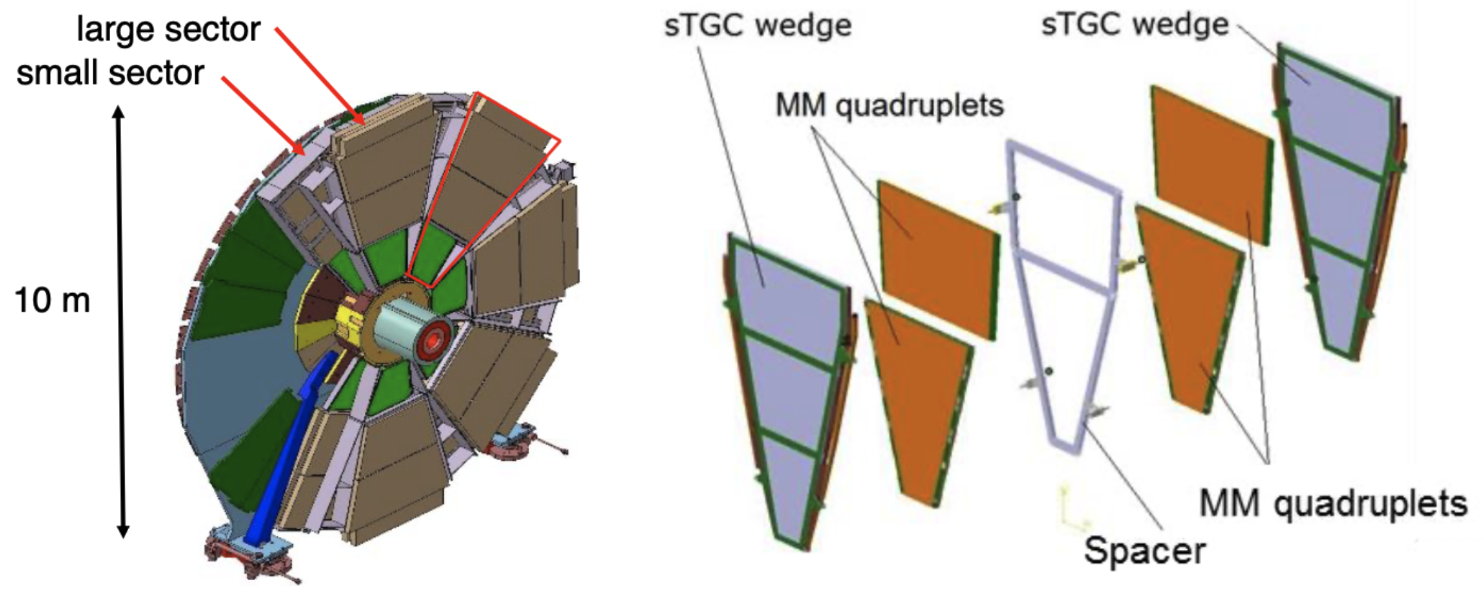
\includegraphics[clip, width=13cm]{fig/2/nsw-structure.png}
  \caption{NSW の構造\cite{article:NSW}。Large Sector と Small Sector の2種類のチェンバーを交互に配置している。sTGC quadruplet の間に、4 層で構成されている MM が 2 つ挟まれており、合計 16 層で構成されている。}
  \label{fig:NSW}
\end{figure}

small-strip TGC~(sTGC)はTGCと同様のMWPCである。図~\ref{fig:sTGC}に示すようにsTGCはTGCと異なり、ストリップを用いて$\eta$方向の位置座標を、ワイヤーを用いて$\phi$方向の位置座標を測定する。sTGCにはパッドと呼ばれる読み出しカソードがあり、ストリップとパッドでアノードワイヤーを挟む構造になっている。
%パッドを用いて大まかな位置情報を計算し信号を読み出す領域を限定した後、ストリップからの信号を用いてより精密な位置情報の計算を行うことで高速な飛跡再構成を行う。

\begin{figure}[tb]
  \centering
  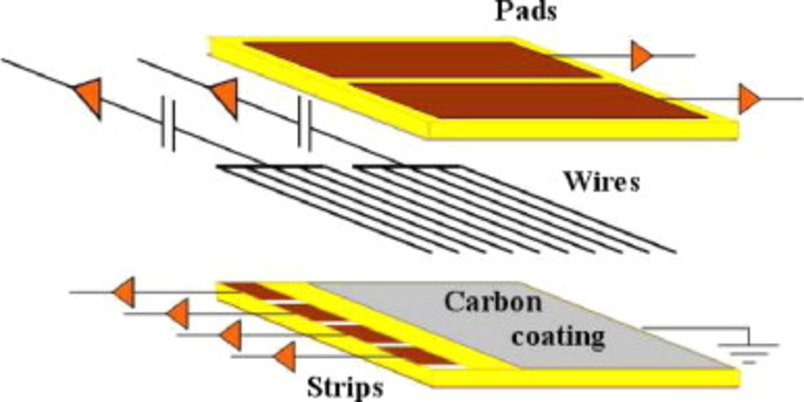
\includegraphics[clip, width=9cm]{fig/2/stgc-structure.pdf}
  \caption{sTGCの断面図~\cite{article:NSW_tech}。 パッド、ストリップを用いて $\eta$ を、ワイヤーを用いて $\phi$ を計算する。}
  \label{fig:sTGC}
\end{figure}

Micromegas~(MM) は、平面の電極と金属のメッシュで構成されている。図~\ref{fig:MM}にMMの概要図を示す。
厚さ5~mmのドリフト領域と128~$\rm{\mu}$mの増幅領域がメッシュで隔てられており、読み出された信号の時間差を用いることで飛跡の$z$方向の情報を再構成することがでる。

\begin{figure}[tb]
  \centering
  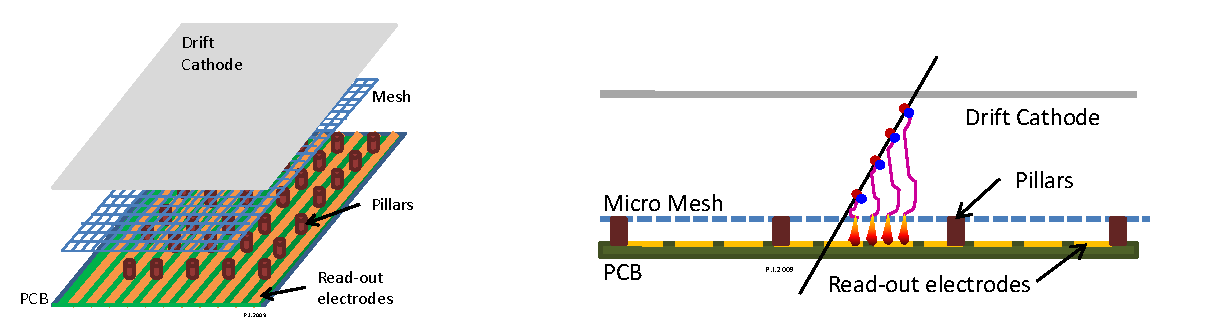
\includegraphics[clip, width=15cm]{fig/2/mm-structure.pdf}
  \caption{MMの概略図~\cite{article:NSW_tech}。メッシュによってドリフト領域と増幅領域に分けられる。ドリフト領域で生成された電子はメッシュを通過し、増幅領域で電場により増幅される。}
  \label{fig:MM}
\end{figure}


\newpage
\section{ATLAS トリガーシステム}
ATLAS実験では、LHCを用いて40~MHzでの頻度で陽子バンチの衝突を行っている。しかし、データ記憶容量の制限が存在するためすべての衝突事象を保存することはできず、現在の制約では事象頻度~(トリガーレート)を数~kHzまで削減する必要がある。
そのため、トリガーシステムと呼ばれる膨大なデータの中から物理として興味のある事象のみを効率よく取得するアルゴリズムを用いて事象選別を行っている。
ATLAS検出器では大きく分けて2段階のトリガーを実装している。1段目にはハードウェアベースの高速処理が可能な初段トリガー、2段目にはソフトウェアベースで精密処理が可能な後段トリガーが実装されている。
トリガーシステムの構成を図~\ref{fig:トリガーの全体像}に示す。

\begin{figure}[tb]
  \centering
  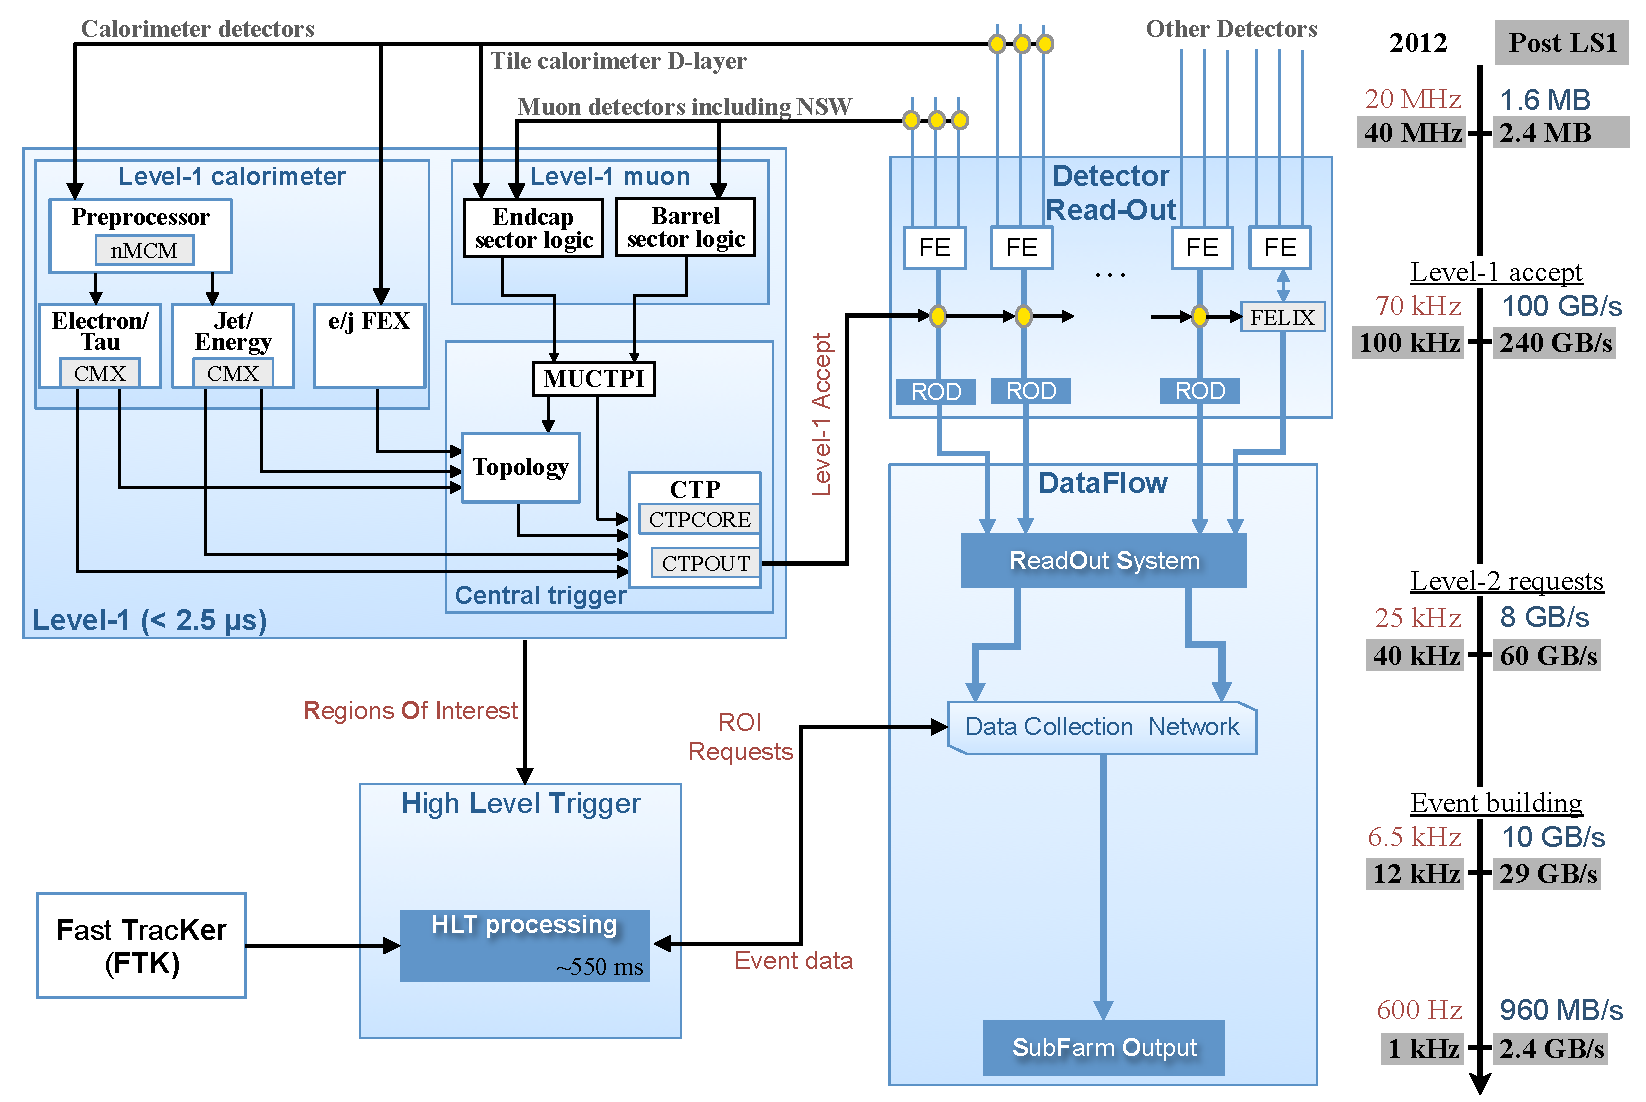
\includegraphics[clip, width=14cm]{fig/3/trigger-nagare2.pdf}
  \caption{Run-3 における ATLAS トリガーシステム及びデータ読み出しの流れ\cite{article:Run3trigger}。トリガーシステムは L1 Trigger LTの 2 段階のトリガーで構成されている。L1 には L1Calo、L1Muon、L1Topo の 3種類が存在する}
  \label{fig:トリガーの全体像}
\end{figure}

\subsubsection{初段トリガー~(L1 Trigger)}\label{L1Topo}
初段トリガーであるL1 Triggerでは、ATLAS検出器から送られてくる40~MHzイベントレートの事象を2.5~$\rm{\mu s}$ 以内にトリガー判定を行い、100~kHzまで落とす必要がある。
高速なトリガー判定を実現するために、Application Specific Integrated Circuit~(ASIC)やField Programmable Gate Array~(FPGA)などの論理回路で構成した電子回路で実装されている。
ASICは特定の用途向けに複数の回路を 1 つにまとめたもので、高速な動作速度や低い消費電力を実現できる一方、回路の修正が困難である。FPGAはASICと同様に特定の処理を行うように設計可能な集積回路で、ASICと比較して処理速度が遅い一方で、何度でも書き換え可能であるというメリットがある。

図\ref{fig:トリガーの全体像}に示すように、L1 Trigger はカロリメータの情報を用いてトリガー判定を行うL1Calo、ミューオン検出器の情報を用いてトリガー判定を行うL1Muonに加え、これらを組み合わせた複合的なトリガーであるCentral Triggerから構成されている。
L1Caloは電磁カロリメータとハドロンカロリメータの情報を統合して、電子/光子と$\tau$候補、ジェット候補の判定を行う。
L1Muonはバレル部の RPC とエンドキャップ部の TGC から情報を受け取り、それぞれ独立にミューオン候補の判定を行う。バレル部とエンドキャップ部で独立に判定された L1Muon の情報はMuon-to-CTP interface~(MUCTPI) で統合される。
その後、L1CaloとL1Muon からの情報はCentral Trigger Processor~(CTP)に送られるのと同時に、TopologyProcessor~(L1Topo) に送られる。L1TopoではL1MuonとL1Caloの情報を組み合わせて、それぞれの情報から複合的な判定を行う。
最後に L1Muon、L1Calo、L1Topo の情報はCTPに集められ、100~kHzに収まるようにプリスケールがかけられた後、トリガーが発行される。

\subsubsection{後段トリガー~(High-Level Trigger:HLT)}
HLTでは、L1 Triggerでの粒子のトリガー判定の領域に対して、ミューオン、電子、光子などをソフトウェアを用いたオフライン解析に近いアルゴリズムで再構成することで精密なトリガー判定を行う。
Level-1 Triggerで用いられなかった内部飛跡検出器の情報、MDTやなどの精密測定用のミューオン検出器及び、カロリメータの情報などを用いて、飛跡再構成やより高精度な $E_T$、$p_T$ の計算を行う。トリガーレートはHLTを用いて最終的に数~kHzまで削減される。

\subsection{トリガーメニュー}
ATLAS実験で用いられているトリガーシステムでは、限られたレートの中に必要な情報を収めなければならない。L1 TriggerとHLTにはそれぞれに条件が設定されている。これをトリガーアイテムと呼ぶ。
例として、L1Muonではミューオンの横方向運動量$p_{\rm{T}}$に閾値を設定したトリガーアイテムがある。基本的に低い$p_{\rm{T}}$のミューオンを取得することが物理としては望ましいが、取得できるレートとの兼ね合いから、この$p_{\rm{T}}$閾値が決定されている。
より低い$p_{\rm{T}}$のミューオンを取得するためには、レートを抑える工夫が必要であり、L1Muonでは同時に複数のミューオンのが存在するといった条件をかけることでレートを減らし、低い$p_{\rm{T}}$のミューオンを取得可能なトリガーアイテムが存在する。
そして、L1 TriggerとHLTのトリガーアイテムを組み合わせたものをトリガーチェインを呼び、トリガーチェインとトリガーレートの配分をまとめたものがトリガーメニューである。表~\ref{triigermenu}にRun-3におけるのL1Muonのトリガーメニューの一例を示す。

L1 Triggerではハードウェア上に512個のトリガーアイテムが用意されており、そのいずれかが鳴ったときにトリガーが発行される。一方で、HLTではソフトウェアベースのトリガー判定を行うため、トリガーアイテムの個数の制限はない。
L1 TriggerとHLTのトリガーアイテムを組み合わせたトリガーチェインは大きく分けて2種類であり、物理解析に使用されるデータの収集のための主要なトリガーであるプライマリートリガーと、効率や性能の評価やモニタリングに使用されるサポートトリガーが存在する。
その中には、新粒子探索に用いる高い$p_{\rm{T}}$の電子やミューオンなどを取得するためのトリガーチェインや、$B$粒子の崩壊などからの低い運動量の粒子を取得するための低い閾値のトリガーチェインなど、多くのトリガーが用意されている。
しかし、トリガーレートに制限があるため、すべてのトリガーを使ってデータを取得することは現実的にはできない。そのため、ATLAS実験のトリガーシステムにはプリスケールファクターと呼ばれる値がトリガーアイテムごとに設定されており、そのトリガーアイテムがトリガー発行する割合を下げることができるため、高いレートになってしまうトリガーに関してもレートを下げてトリガー発行することが可能になっている。

\begin{table}[]
    \caption{Run-3におけるプライマリーミューオントリガーのメニューの一例~\cite{article:Run3trigmenu}。L1及びHLTのプライマリートリガーのトリガーアイテムとRun-3で予想されるレートを示す。}
    \label{triigermenu}
    \centering
    %\begin{tabular}{|c|c|c|c|c|c|c|c|c|c|c|c|c|c|c|c|c|c|c|c|c|c|c|c|}
    \begin{tabular}{|c|c|c|r|}
    \hline
        L1 Target & Category & Trigger item & Rate\\
        \hline
        MU  & L1 & L1$\_$MU14FCH & 17~kHz\\
        \hline
            &HLT 1mu isolation & HLT$\_$mu26$\_$ivarmedium& 195~Hz\\
            &        & HLT$\_$mu24$\_$ivarmedium & 229~Hz\\
        \hline
            &HLT 1mu& HLT$\_$mu26$\_$ivarmedium & 38~Hz\\
            &       & HLT$\_$mu60$\_$0eta105$\_$msonly & 10~Hz\\
            &       & HLT$\_$mu80$\_$msonly$\_$3layersEC & 8~Hz\\
        \hline
            &HLT 2mu & HLT$\_$mu22$\_$mu8noL1 & 45~Hz\\
            &       & HLT$\_$mu20$\_$ivarmedium$\_$mu8noL1 & 19~Hz\\
            &       & HLT$\_$mu20$\_$ivarmedium$\_$mu4noL1$\_$10invmAB70 & 12~Hz\\
            &       & HLT$\_$2mu50$\_$msonly & 6~Hz\\
        \hline
            &HLT 3mu    & HLT$\_$mu20$\_$2mu4noL1 & 6~Hz\\
        \hline
        \hline
        2MU & L1        & L1$\_$2MU8F & 2.2 kHz\\
        \hline
            & HLT 2mu   & HLT$\_$2mu14 & 23 Hz\\
            &           & HLT$\_$mu10$\_$ivarmedium$\_$mu10$\_$10invmAB70 & 15~Hz\\
        \hline
        \hline
        2MU & L1 & L1$\_$MU10BOM & 0.9~kHz\\
        \hline
            & HLT 2mu & HLT$\_$2mu10$\_$l2mt & 1~Hz\\
        \hline
        \hline
        3MU &L1 & L1$\_$3MU5VF & 0.2~kHz\\
        \hline
            &HLT 3mu & HLT$\_$3mu6 & 5~Hz\\
            &        &HLT$\_$3mu6$\_$msonly &27~Hz\\
        \hline
        \hline
        4MU & L1 & L1$\_$4MU3V & 0.4~kHz\\
        \hline
            & HLT 4mu & HLT$\_$4mu4 & 1~Hz\\
        \hline
    \end{tabular}
\end{table}


%\begin{figure}[b]
%  \centering
%  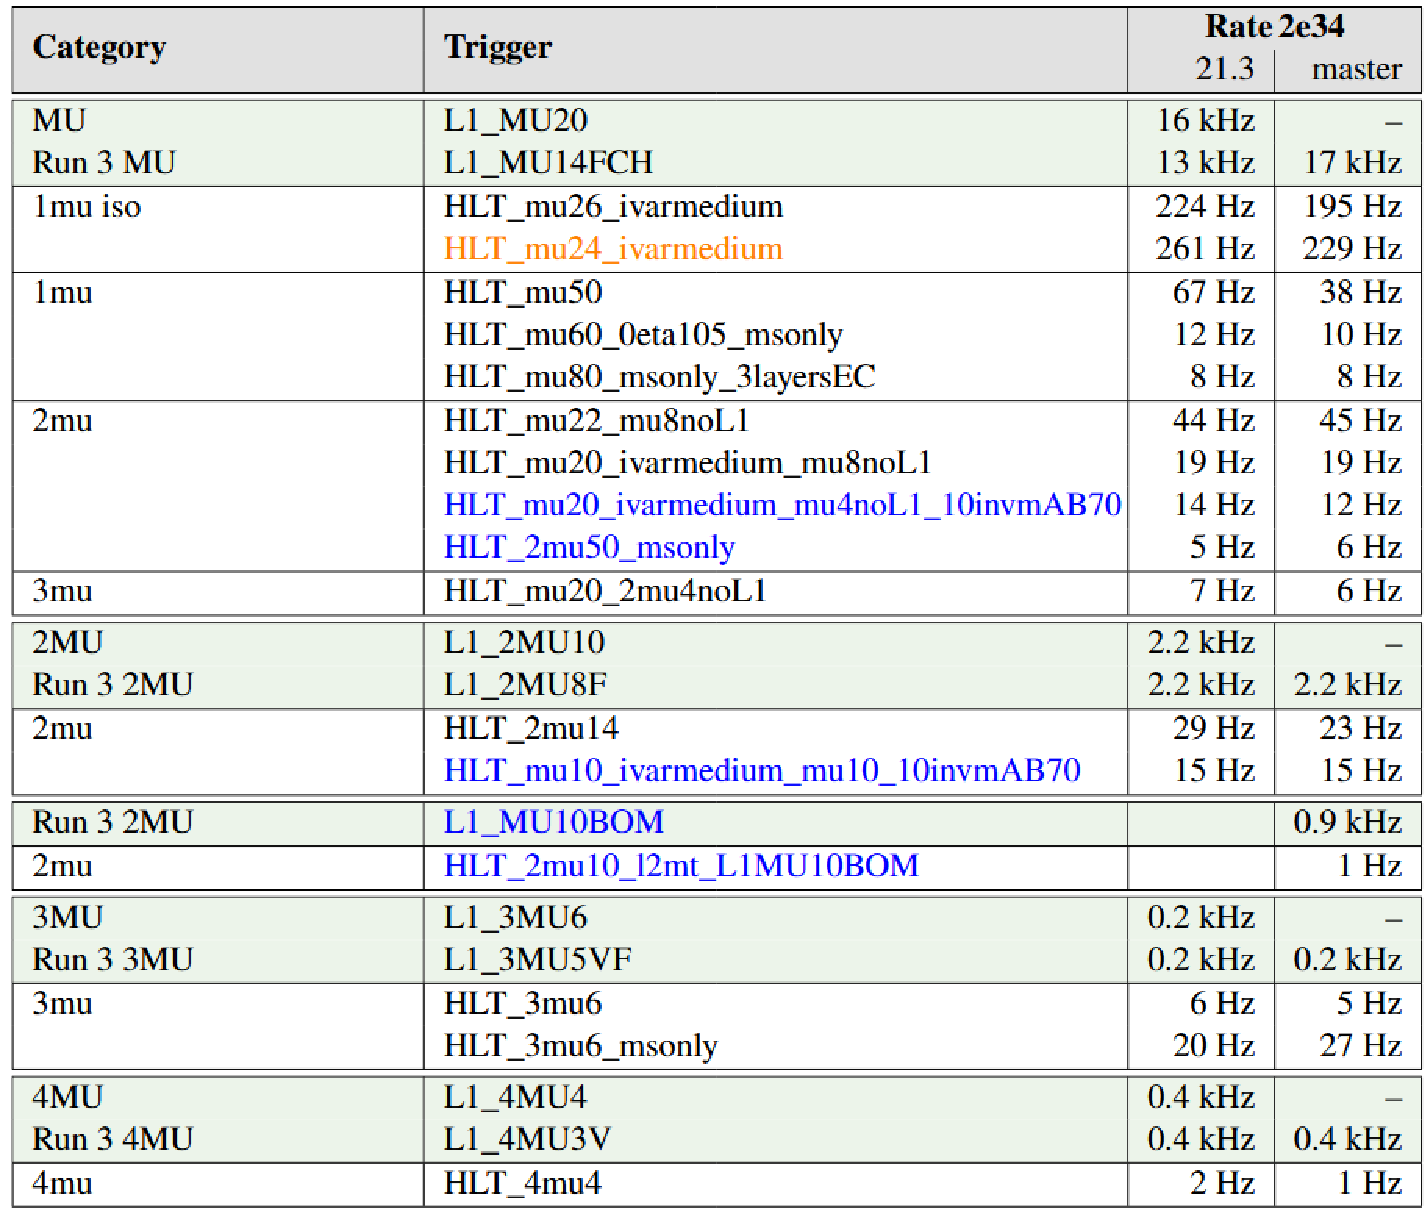
\includegraphics[clip, width=14cm]{fig/2/muon_trigger_menu.pdf}
%  \caption{Run-3 におけるプライマリーミューオントリガーのメニュー\cite{article:Run3trigmenu}。}
%  \label{fig:muon_trigger_menu.pdf}
%\end{figure}

